%% Submitted to: Mathematics (MDPI)
%% Class: Definitions/mdpi  (download from https://www.mdpi.com/authors/latex)

\documentclass[mathematics,article,submit,pdftex,moreauthors]{Definitions/mdpi}

\firstpage{1}
\makeatletter
\setcounter{page}{\@firstpage}
\makeatother
\pubvolume{1}
\issuenum{1}
\articlenumber{0}
\pubyear{2026}
\copyrightyear{2026}
\datereceived{}
\daterevised{}
\dateaccepted{}
\datepublished{}

\usepackage{adjustbox}
\usepackage{algorithm}
\usepackage{algpseudocode}
\usepackage{pifont}
\newcommand{\cmark}{\ding{51}}
\newcommand{\xmark}{\ding{55}}

\newtheorem{claim}{Claim}[section]

\newcommand{\orcidauthorA}{0000-0001-6384-8840}
\newcommand{\orcidauthorB}{0009-0005-9746-0058}
\newcommand{\orcidauthorC}{0000-0002-3895-688X}

\Title{The Missing Signal: Gradient Injection Recovers $O(n^2)$ Residual Decoding in GNNs}

\Author{
  Elad Shoham $^{1,*}$\orcidA{},
  Havana Rika $^{2}$\orcidB{}
  and Dan Vilenchik $^{1,*}$\orcidC{}
}

\AuthorNames{Elad Shoham, Havana Rika and Dan Vilenchik}

\address{
  $^{1}$ \quad Department of Software and Information Systems Engineering,
  Ben-Gurion University of the Negev,
  Beer-Sheva 8410501, Israel; shellad@post.bgu.ac.il, vilenchi@bgu.ac.il \\
  $^{2}$ \quad The Academic College of Tel Aviv-Yaffo,
  Tel Aviv 61083, Israel;
  havanari@mta.ac.il
}

\corres{Correspondence: shellad@post.bgu.ac.il; vilenchi@bgu.ac.il}


  % Residual decoding algorithms repeatedly score the current elements, prune one
  % candidate, and update the residual state. Classical implementations are efficient
  % because their scores are built from additive statistics such as degree: after a
  % deletion, each surviving score changes by a local correction that can be applied in
  % $O(n)$ time, yielding $O(n^2)$ total decoding cost. A Graph Neural Network (GNN) score does not have this
  % property automatically. Once the score passes through nonlinear activations such as
  % $\tanh$ or sigmoid, equal changes in the underlying statistic need not induce equal
  % changes in the output---the gap between $\tanh(6)$ and $\tanh(5)$ differs from the
  % gap between $\tanh(2)$ and $\tanh(1)$---so no fixed additive correction can update
  % the score after a deletion. The standard adaptive alternative is to rerun the full network after
  % every deletion, inflating decoding cost to $O(n^3)$.
  % We use the gradient induced by the unsupervised clique objective as an
  % update-compatible residual signal, and validate this on \textsc{Max-Clique}
  % using planted-clique instances. After each vertex deletion, each surviving gradient
  % coordinate changes by a local, maintainable quantity, updatable in $O(n)$ per step.
  % Supplying this live gradient to a lightweight learned updater recovers $O(n^2)$
  % decoding, matching the $O(n^3)$ rerun baseline on Easy and Medium regimes.
  % Zero-shot evaluation on six real-world graph benchmarks confirms that gradient
  % injection consistently outperforms score-only updating, with a quality--efficiency
  % gap remaining on the most heterogeneous graphs.
  
\abstract{%
  Residual decoding algorithms repeatedly score the current elements, prune one
  candidate, and update the residual state. Classical implementations are efficient
  because their scores are built from locally maintainable statistics such as degree:
  after a deletion, surviving scores change by local corrections, giving $O(n^2)$
  total decoding cost. A Graph Neural Network (GNN) score does not automatically have
  this property. After nonlinear activations such as $\tanh$ or sigmoid, equal changes
  in the underlying statistic need not induce equal changes in the output, so no fixed
  additive correction can generally update the score after a deletion. The standard
  adaptive alternative is to rerun the full network after every deletion, inflating
  decoding cost to $O(n^3)$. We show that, for \textsc{Max-Clique}, the gradient of an
  unsupervised clique objective provides an update-compatible residual signal. After
  each vertex deletion, every surviving gradient coordinate changes by a local,
  maintainable quantity, updatable in $O(n)$ per step. Supplying this live gradient to
  a lightweight learned updater recovers $O(n^2)$ decoding and matches the $O(n^3)$
  rerun baseline on Easy and Medium planted-clique regimes. Zero-shot evaluation on
  six real-world graph benchmarks confirms consistent gains over score-only updating.
}

\keyword{%
  graph neural networks;
  combinatorial optimization;
  Max-Clique;
  residual decoding;
  unsupervised learning
}

\MSC{68T07; 68R10; 90C35}

% ================================================================
\begin{document}
\maketitle
% ================================================================

% ================================================================
\section{Introduction}
% ================================================================

Many combinatorial algorithms have the same residual structure: score the current
objects, remove or select one, update the remaining instance, and repeat. The loop is
efficient when the maintained statistic has a local update rule. Degree is the
canonical example: after deleting a vertex, each surviving degree changes by a local
adjacency-dependent correction, so all degrees can be updated in $O(n)$ time and the
whole dense-graph deletion loop costs $O(n^2)$.

We study residual decoding for \textsc{Max-Clique}: given a graph, find a largest
set of pairwise adjacent vertices. The problem is NP-hard, and its worst-case approximation is also hard~\citep{karp1972,feige1996approximating,hastad1999}, but practical algorithms and heuristics exploit structure through branch-and-bound, greedy pruning,
local-degree refinement, spectral methods for average-case recovery, and continuous formulations
\citep{alon1998,wu2015review,gibbons1997continuous,marino2024short}. In the
planted-clique setting used here, a clique is hidden inside a random background graph;
the decoder must recover it by preserving the planted vertices during pruning.

Graph Neural Networks (GNNs) offer a learned analogue of these hand-designed scoring heuristics
\citep{karalias2020,min2022,garmendia2024}. Prior interpretability work shows that,
for \textsc{Max-Clique}, GNN rankings often collapse to a degree-like concept
\citep{ShohamHRV26}. This suggests a simple hope: replace the hand-designed residual
statistic with the learned GNN score and keep the same efficient deletion loop.

The obstacle is update compatibility. A classical statistic such as degree changes
additively under deletion, but a GNN score that has passed through nonlinear layers
need not. Equal changes in an underlying statistic can induce unequal score changes,
so a fixed local correction cannot generally update the score after a deletion. The
standard adaptive alternative is to rerun the full GNN on every residual graph, which gives fresh
scores but raises decoding from $O(n^2)$ to $O(n^3)$.

This leads to the central question: \textbf{Can a learned residual decoder match
  the solution quality of rerunning the GNN after each deletion while recovering the
$O(n^2)$ update structure of classical residual algorithms?}

Our answer is to separate the learned score from the maintained residual state. The
raw score is not reliably updatable, but the probability-space gradient of the clique
objective is: after a vertex is deleted, each surviving gradient coordinate changes
by a local correction. We therefore feed a cached, incrementally maintained gradient
to a lightweight updater $U_\theta$. The updater still learns how to modify scores,
but it acts on a live residual signal rather than on stale nonlinear scores alone.

\subsection{Contributions}

Our main contribution is an update-compatible neural residual decoder for
\textsc{Max-Clique}. The decoder runs the GNN once, maintains the probability-space
clique gradient after each deletion, and feeds this live residual signal to a small
learned updater. The gradient coordinate,
$\nabla_p\mathcal{L}_{\mathrm{clique}}$, changes locally after each deletion and is
maintainable in $O(n)$ time by cached sufficient statistics, recovering $O(n^2)$
total decoding cost after the initial GNN pass.

Empirically, we introduce U-LPR (Updatable Least Probable Removal), which runs the
GNN once and updates scores through a lightweight learned updater $U_\theta$. We test
a score-only updater (\textsc{SGNN+U}) against a gradient-injected updater
(\textsc{SGNN+GU}) and train both with Self-Imitation Training (SIT), where the
student imitates a rerun-based teacher; Figure~\ref{fig:decoder_overview}
summarizes these decoder variants. Our findings are:
\begin{itemize}
  \item \textbf{Recovery quality and running time.} \textsc{SGNN+GU} under SIT training
    achieves approximation, overlap, and exact recovery of $1.00$ on Easy and
    Medium regimes at $O(n^2)$ cost, matching the $O(n^3)$ rerun baseline with a roughly
    $1.5\times$ wall-clock speedup in our timing table.
  \item \textbf{Empirical importance of the gradient channel.} Removing the gradient leaves
    \textsc{SGNN+U} unable to maintain rerun-quality U-LPR decoding on Medium
    instances, indicating that gradient injection is empirically critical for this
    updater architecture, not merely a helpful signal.
  \item \textbf{Low-degree pruning behavior.} Deletion diagnostics show that the
    successful updater follows a coarse residual low-degree rule: it avoids deleting
    vertices above the 15th percentile of residual degree, rather than sorting
    vertices by exact degree.
  \item \textbf{Real-world generalization.} Evaluated zero-shot on six real-world
    graph benchmarks from~\citet{ShohamHRV26}, \textsc{SGNN+GU} U-LPR substantially
    outperforms the score-only updater on all datasets and approaches the $O(n^3)$
    rerun baseline on four of six. On heterogeneous graphs (Twitter, Facebook), a
    quality--efficiency gap remains, suggesting logit-space residual signals as a
    direction for future work.
\end{itemize}

\begin{figure}[H]
  \centering
  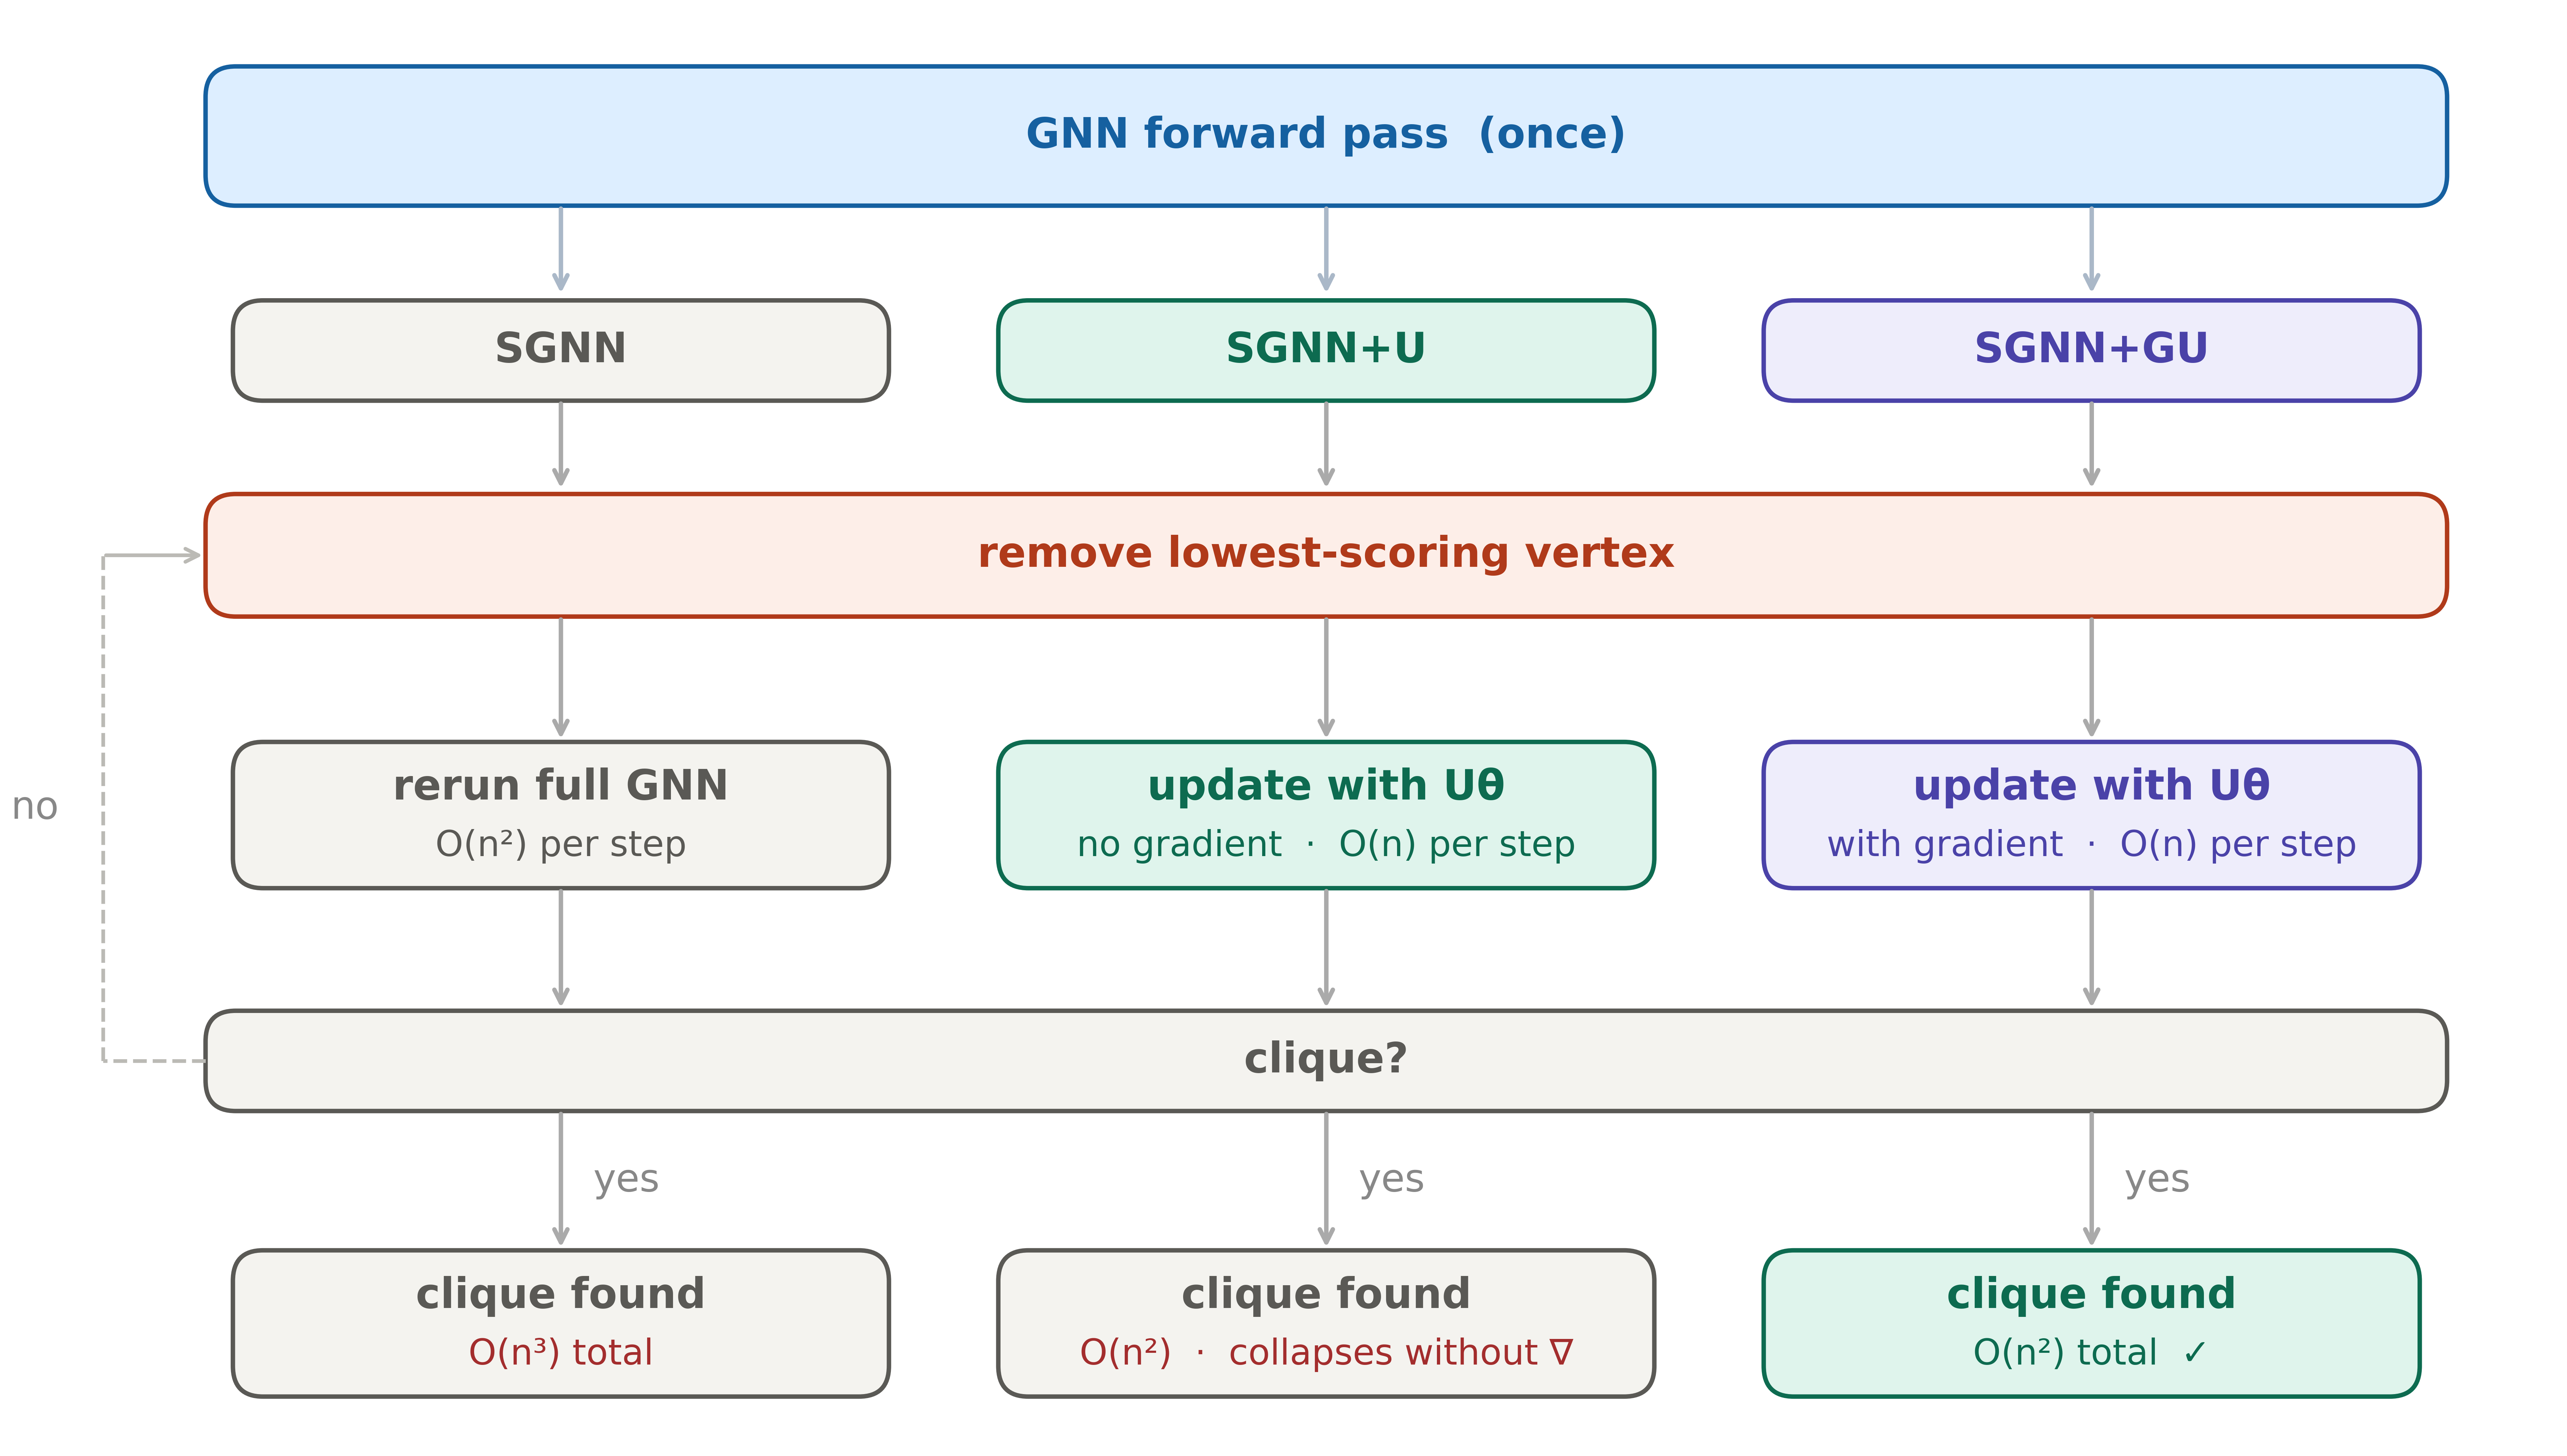
\includegraphics[width=0.92\textwidth]{decoder_figure.png}
  \caption{Overview of the three neural decoder variants. \textsc{SGNN} uses the backbone
    scores directly, \textsc{SGNN+U} adds an incremental score updater without gradient
    information, and \textsc{SGNN+GU} supplies the updater with a cached residual gradient.
    The gradient channel supplies the locally maintainable residual signal used by the
  learned updater in the $O(n^2)$ decoder.}
  \label{fig:decoder_overview}
\end{figure}

\paragraph{Paper organization.}
The remainder of the paper is organized as follows. Section~\ref{sec:related}
positions the work relative to GNN-based combinatorial optimization,
\textsc{Max-Clique} algorithms, and planted-clique recovery. Section~\ref{sec:method}
defines the planted-clique setting, decoder variants, datasets, model architecture,
training objectives, and evaluation protocol. Section~\ref{sec:theory} gives the
update-compatibility analysis that motivates gradient injection and cached
maintenance. Section~\ref{sec:experiments} reports synthetic and real-world results,
including timing and pruning diagnostics. Sections~\ref{sec:discussion}
and~\ref{sec:conclusions} discuss limitations, future directions, and the main
conclusions.

% ================================================================
\section{Background and Related Work}
\label{sec:related}
% ================================================================

Our backbone is a standard message-passing neural network (MPNN)~\citep{xu2019}.
Although MPNN expressiveness is bounded by the 1-WL test~\citep{xu2019,morris2019},
expressiveness is not the bottleneck studied here. The question is algorithmic:
a score may be informative on the current graph but still unsuitable for cheap
maintenance after the graph changes.

This interface is often implicit in neural combinatorial optimization. GNN-based
heuristics have been developed for \textsc{Max-Clique}, \textsc{Max-Cut},
\textsc{Max-Independent-Set}, and related problems
\citep{karalias2020,min2022,schuetz2022,garmendia2024,tonshoff2021graph}, with
training procedure and state representation playing an important role
\citep{wang2023unsupervised,garmendia2024}. These works show that learned scores can
be useful; we ask whether such scores remain usable inside an adaptive residual
loop.

\textsc{Max-Clique} is a natural setting for this question because its classical
heuristics make the maintained state explicit. Algorithms range from exact
enumeration and branch-and-bound to greedy pruning, local search, and continuous
formulations~\citep{bron1973algorithm,wu2015review,gibbons1997continuous,marino2024short}.
In planted clique, the asymptotic picture is more structured: degree thresholding
succeeds for sufficiently large planted cliques~\citep{kucera1995}, spectral
methods recover cliques around the $\sqrt n$ scale~\citep{alon1998}, and repeated
low-degree removal improves the practical recovery boundary~\citep{feige2010,dekel2014}.
Below the conjectured polynomial-time recovery threshold, planted-clique hardness
assumptions support lower bounds across several statistical tasks
\citep{manurangsi2021,hajek2015}.

The learning-to-rank study of \citet{ShohamHRV26} used these regimes to build a
difficulty-aware \textsc{Max-Clique} benchmark and showed that GNN embeddings
collapse to a degree/row-sum ranking concept. We inherit that benchmark structure
but ask a different question: not only whether the initial GNN ranking is accurate
at $t=0$, but whether the information it encodes can be maintained cheaply as
vertices are deleted. This shifts the focus from static ranking quality to the
state variable used by the decoder.

We use deletion diagnostics only to interpret the learned pruning behavior. Unlike
prior concept-probing work~\citep{ShohamHRV26,shoham2026sat,kim2018,schut2023bridging},
our claim is not that the updater explicitly represents degree as an extracted
concept, but that its deletion choices follow a coarse residual low-degree rule.

This connects our work to methods that feed algorithmic state or intermediate
predictions back into a neural solver. OptGNN proved that polynomial-sized MPNNs can
implement SDP gradient descent for Max-CSPs~\citep{yau2023}; QRF-GNN feeds
intermediate GNN predictions back as dynamic node features and requires a full GNN
forward pass at each round~\citep{gaile2024}; and unrolled optimization networks
make each layer correspond to a meaningful algorithmic step~\citep{monga2021,hadou2025}.
Our gradient channel differs in what is fed back (objective gradient
rather than prediction outputs) and in how it is maintained (a cached $O(n)$
update per deletion rather than a full GNN rerun): the maintained signal is not
merely another recurrent feature, but the local objective change that remains cheaply
updatable after pruning.

Lastly, this also connects the training problem to imitation learning for combinatorial
search~\citep{liu2021}. In our setting, the imitated policy is a rerun-based
residual decoder and the learned policy is an incremental updater. Section~\ref{sec:training_objective}
defines this self-imitation objective; the key empirical question is whether the
student can imitate the rerun trajectory from stale scores alone, or whether it
needs the maintained gradient state.

\section{Materials and Methods}
\label{sec:method}
% ================================================================

\subsection{Problem Setting}
\label{sec:problem}

We focus on \textsc{Max-Clique}: given a graph $G=(V,E)$, find the largest subset
$C \subseteq V$ such that all pairs in $C$ are adjacent. Let $A$ be the adjacency
matrix and let $B=\mathbf{1}\mathbf{1}^{\top}-I-A$ be the non-edge matrix. For a
binary vector $x\in\{0,1\}^n$ with $\|x\|_0=k$, the quantity $x^\top A x$ equals
twice the number of induced edges, while $x^\top Bx$ counts twice the number of
induced non-edges. Thus, a size-$k$ clique is characterized by
\[
  x^\top A x = 2\binom{k}{2}
  \qquad\text{and equivalently}\qquad
  x^\top Bx = 0 .
\]
This quadratic view is standard in learning-based analyses of clique recovery and
will also be used below to define the unsupervised clique objective
\citep{ShohamHRV26,min2022,karalias2020}.

We evaluate on the planted-clique distribution $G(n,\tfrac{1}{2},k)$: first sample
an Erd\H{o}s--R\'enyi graph on $n$ vertices where each edge is included
independently with probability $1/2$, then choose $k$ vertices uniformly at random
and add all missing edges among them. The goal is to recover a large valid clique,
ideally the planted clique $C^\star$. This distribution is a standard testbed for
studying the statistical and computational limits of clique recovery, and it has
also been used in recent neural clique-recovery benchmarks
\citep{kucera1995,alon1998,feige2010,dekel2014,ShohamHRV26}.

\subsubsection{Decoders}

A natural family of decoders for this problem is the \emph{residual loop}: score all
vertices, remove the lowest-scoring one, and repeat until the remaining set forms a
clique. Classical Least Degree Removal (LDR) instantiates this loop with residual
degree. The learning-to-rank variant of~\citet{ShohamHRV26} replaces degree
with a learned GNN probability, giving Least Probable Removal (LPR). In this paper,
we use that lineage mainly to define the updatable decoder, U-LPR. The main table
therefore does not include LDR or LPR as separate rows; in the Hard-regime
discussion, we cite LDR only as a classical reference point.

We evaluate three decoders:
\begin{itemize}
  \item \textbf{Top-$k$}: a non-iterative baseline that runs the GNN once, ranks
    vertices by score, and greedily removes the lowest score without updated the scores, until a clique remains (corresponding to the original decoding strategy
    of~\citet{karalias2020}). $O(n^2)$.
  \item \textbf{Rerun}: reruns the full GNN after every deletion to produce fresh
    scores. The only $O(n^3)$ decoder, serving as the adaptive upper bound.
  \item \textbf{U-LPR} (Updatable Least Probable Removal): runs the GNN once and
    applies a learned MLP updater $U_\theta$ after each deletion to incrementally
    correct the scores (Algorithm~\ref{alg:gub}). $O(n^2)$.
\end{itemize}

\subsubsection{Datasets and Difficulty Regimes}

We evaluate on synthetic planted-clique instances $G(n,\tfrac{1}{2},k)$ with
$n=1000$ vertices. Each instance is generated by first sampling $k$ uniformly from
the relevant regime interval, then choosing $k$ vertices uniformly at random and
adding all missing edges among them; all remaining edges are sampled independently
with probability $1/2$.

Following~\citet{ShohamHRV26}, the Easy/Medium/Hard labels are derived from the
algorithmic thresholds for planted clique recovery and then calibrated at the fixed
finite graph size. Asymptotically, larger planted cliques give the planted vertices
a visible degree boost: when $k=\Omega(\sqrt{n\log n})$, simple degree-based
ranking succeeds \cite{kucera1995}; when $k=\Omega(\sqrt n)$ but below the degree-ranking threshold,
recovery requires stronger residual or spectral methods \cite{alon1998,feige2020hide}; and around the
$O(\sqrt n)$ scale, the planted clique hardness conjecture predicts that recovery
is computationally intractable~\cite{manurangsi2021,hajek2015,ma2015computational,berthet2013complexity,hazan2011hardness}.

For a fixed $n$, the finite thresholds are obtained empirically as follows. Let
$k_1$ be the smallest clique size for which the Top-$k$ degree heuristic recovers
the planted clique at least $90\%$ of the time. Lower $k$ until the degree-based
residual-removal heuristic falls below $90\%$ success, and denote that cutoff by
$k_2$. Finally, set
$k_3=\lceil 2\log_2 n\rceil$, the typical largest-clique scale in the unplanted
background graph~\citep{bollobas1985}. The full calibrated regions are Easy
$[k_1,n]$, Medium $[k_2+1,k_1-1]$, and Hard $[k_3,k_2]$.

For $n=1000$, this calibration gives $k_1=62$, $k_2=35$, and $k_3=20$. The reported
experiments therefore use the following sampled ranges:
\begin{itemize}
  \item \textbf{Easy} ($k\in[62,100]$): a bounded subset of the full easy region
    $k\ge 62$, where degree-based ranking already succeeds~\citep{kucera1995}.
  \item \textbf{Medium} ($k\in[36,61]$): below the Top-$k$ degree threshold but
    still recoverable by stronger residual or spectral methods such
    as repeated low-degree removal and AKS~\citep{alon1998,feige2010}.
  \item \textbf{Hard} ($k\in[20,35]$): near the background clique scale and below
    the empirical residual-method threshold, where no polynomial-time method is
    known to recover the planted clique reliably~\citep{manurangsi2021}.
\end{itemize}

\subsubsection{Real-World Datasets}
\label{sec:realworld_data}

To assess generalization beyond the planted-clique distribution, we also evaluate
on six real-world graph benchmarks used in~\citet{ShohamHRV26}.
Twitter, Collab, and IMDB Binary are graph-classification benchmarks from the
TUDataset collection~\citep{Morris+2020,10.1145/2783258.2783417}.
com-youtube and com-orkut are large community-network graphs from the SNAP
repository~\citep{youtube-orkut,datasets}.
Facebook consists of ego networks from the same
repository~\citep{facebook,datasets}.
Full dataset statistics are given in Table~\ref{tab:datasets}. Models are trained
on planted-clique instances as described in Section~\ref{sec:training} and evaluated
zero-shot on the real-world graphs without any re-training or fine-tuning. The
$O(n^3)$ SGNN Rerun baseline is reproduced from~\citet{ShohamHRV26}; our
contribution is the $O(n^2)$ U-LPR results. The three task metrics are defined in
Section~\ref{sec:evaluation_methodology} and applied identically.

\begin{table}[H]
  \caption{Dataset statistics. $n$ is the mean number of nodes per graph ($\pm$ std);
    $k$ is the range of clique sizes found across graphs in the dataset. Synthetic
    datasets are generated as described in Section~\ref{sec:problem}. Real-world
    datasets are per-community or ego subgraphs; small mean sizes alongside large
  standard deviations reflect power-law community-size distributions.}
  \label{tab:datasets}
  \centering
  \resizebox{0.82\textwidth}{!}{%
    \begin{tabular}{lrccc}
      \toprule
      Dataset & Graphs & $n$ (mean$\pm$std) & $k$ range & Type \\
      \midrule
      \multicolumn{5}{l}{\emph{Synthetic planted-clique}} \\
      Easy ($n=1000$)    & 1000  & $1000$           & $[62,100]$  & Random \\
      Medium ($n=1000$)  & 1000  & $1000$           & $[36,61]$   & Random \\
      Hard ($n=1000$)    & 1000  & $1000$           & $[20,35]$   & Random \\
      \midrule
      \multicolumn{5}{l}{\emph{Real-world benchmarks~\citep{ShohamHRV26}}} \\
      com-youtube  & 16386 & $7.8{\pm}42.2$  & $[2,12]$    & Real \\
      IMDB Binary  & 1000  & $19.8{\pm}10$   & $[4,30]$    & Real \\
      com-orkut    & 5000  & $215{\pm}320$   & $[3,50]$    & Real \\
      Collab       & 5000  & $74.5{\pm}62$   & $[4,239]$   & Real \\
      Twitter      & 973   & $131{\pm}64$    & $[2,70]$    & Real \\
      Facebook$^\dagger$ & 10 & $416{\pm}329$ & $[7,69]$   & Real \\
      \bottomrule
  \end{tabular}}
  \smallskip\par\noindent\small
  $^\dagger$ Ten graphs only; results are indicative.
\end{table}

\subsection{Model Architecture}
\label{sec:architectures}

We evaluate three model families: \textsc{SGNN}, \textsc{SGNN+U}, and \textsc{SGNN+GU}. All share the same
message-passing backbone with $L=4$ steps, hidden dimension $64$, and
$\sigma=\tanh$. The input feature is a scalar liveness indicator; no degree,
clique-membership, or structural feature is provided. The backbone aggregates and
updates as
\[
  q_v^{(\ell)} = \frac{1}{n-1}\sum_{u\in\mathcal{N}(v)} h_u^{(\ell)},
  \qquad
  h_v^{(\ell+1)} = \sigma\!\left(M_{\mathrm{upd}}\!\left[h_v^{(\ell)},
  q_v^{(\ell)}\right]\right),
\]
\[
  s_v = W_{\mathrm{out}} h_v^{(L)} + b_{\mathrm{out}},
  \qquad
  p_v = \operatorname{sigmoid}(s_v),
\]
where $M_{\mathrm{upd}}$ is a two-layer MLP and $p_v \in (0,1)$ is the vertex
probability used by the clique objective. \textsc{SGNN} uses this backbone alone. \textsc{SGNN+U} and
\textsc{SGNN+GU} add a lightweight MLP updater $U_\theta$ that corrects surviving scores
after each deletion of $v^*$:
\[
  s_i \leftarrow s_i + U_\theta(s_i,\, s_{v^*},\, A_{iv^*},\, \gamma_i,\,
  \gamma_{v^*}),
\]
where $\gamma_i, \gamma_{v^*}$ are gradient channels that differ between variants.
For \textsc{SGNN+U}, $\gamma_i = \gamma_{v^*} = 0$. For \textsc{SGNN+GU},
\[
  \gamma_i = g_i = \frac{\partial \mathcal{L}_{\mathrm{clique}}}{\partial p_i},
  \qquad
  \gamma_{v^*} = g_{v^*} = \frac{\partial \mathcal{L}_{\mathrm{clique}}}{\partial
  p_{v^*}},
\]
maintained via cached sufficient statistics updated in $O(n)$ per deletion
(Section~\ref{sec:cached_maintenance}). Since $U_\theta$ is a two-hidden-layer MLP
of fixed width (hidden dimension $64$), each application costs $O(1)$ in model size,
so $n$ updater calls contribute $O(n)$ total to the decoding cost, preserving the
$O(n^2)$ bound.

\subsection{Training Objective}
\label{sec:training_objective}

All models are trained from the unsupervised clique objective
\begin{equation}
  \mathcal{L}_{\mathrm{clique}}(p; A)
  =
  -p^\top A p
  +
  p^\top B p,
  \label{eq:clique_loss}
\end{equation}
where $p_i=\operatorname{sigmoid}(s_i)$ and
$B=\mathbf{1}\mathbf{1}^\top-I-A$ is the complement adjacency matrix without
self-loops. The first term rewards probability mass on edges, while the second
penalizes probability mass assigned to non-edges.
% Importantly, the objective does not use the planted clique size $k$; $k$ is used only to generate instances and to evaluate recovery against the planted clique.

For an alive set $S\subseteq V$, we write $p_i=0$ for $i\notin S$ and restrict
$A$ and $B$ to the current residual graph by masking deleted vertices. The gradient
of~\eqref{eq:clique_loss} with respect to the probability vector is
\begin{equation}
  g
  =
  \nabla_p \mathcal{L}_{\mathrm{clique}}
  =
  -2Ap + 2Bp .
  \label{eq:clique_gradient}
\end{equation}
This is the residual signal supplied to \textsc{SGNN+GU}. If $p_i=\sigma(z_i)$, then the backpropagation gradient with respect to logits would
be
\[
  \nabla_z \mathcal{L}_{\mathrm{clique}}
  =
  \nabla_p \mathcal{L}_{\mathrm{clique}} \odot p \odot (1-p).
\]
We do not use this logit gradient as the updater input. The factor $p_i(1-p_i)$
becomes small when $p_i$ is close to $0$ or $1$, which would suppress the residual
signal in saturated regions. Thus, \textsc{SGNN+GU} receives the unsaturated
probability-space gradient in Eq.~\eqref{eq:clique_gradient}.

\subsubsection{Objective Training (OBJ)}

$\mathcal{L}_{\mathrm{train}} = \mathcal{L}_{\mathrm{clique}}$. Under OBJ, the
loss is applied to the backbone scores on the original graph only; no residual
deletion trajectory is unrolled. Consequently, the updater $U_\theta$ receives no
training signal, and the putative \textsc{SGNN+U}+OBJ and \textsc{SGNN+GU}+OBJ
variants reduce to the backbone-only \textsc{SGNN}+OBJ model. We therefore omit
separate OBJ updater ablations.

\subsubsection{Self-Imitation Training (SIT)}

SIT adds an imitation loss that directly supervises the incremental decoder. At each
step $t$, a rerun-based teacher reruns the GNN on the current residual graph $G_t$
and selects the lowest-scoring vertex $v^t_{\mathrm{teach}}$. A student---running
the GNN only once and updating scores incrementally via $U_\theta$---is penalised
for disagreeing:
\begin{equation}
  \mathcal{L}_{\mathrm{SIT}} = \frac{1}{T} \sum_{t=0}^{T-1}
  \mathrm{CE}_{\mathrm{softmax}}\!\left(-\tilde{s}^{(t)}_{V(G_t)},\;
  v^t_{\mathrm{teach}}\right),
  \qquad
  \mathcal{L}_{\mathrm{train}} = \mathcal{L}_{\mathrm{clique}} +
  \mathcal{L}_{\mathrm{SIT}}.
  \label{eq:sit_loss}
\end{equation}
The minus sign converts the teacher's minimum-score removal rule into a standard
softmax classification target: vertices with lower student scores receive larger
logits in the cross-entropy loss.
For \textsc{SGNN+U}, $U_\theta$ receives no gradient signal and is trained with
$\gamma_i = \gamma_{v^*} = 0$. For \textsc{SGNN+GU}, the cached gradient is updated in
$O(n)$ after each teacher removal before being passed to $U_\theta$. SIT uses
$T=300$ teacher removals per instance during offline training. SIT incurs a
one-time offline distillation cost of $O(T \cdot n^2)$ per training instance due
to teacher reruns; this is not part of inference.
% and is standard practice in imitation learning.
All $O(n^2)$ claims therefore refer to
decoding after training, where the GNN is run once and the updater is applied
incrementally. Algorithm~\ref{alg:sit_training} gives the complete training step.

\subsubsection{Cached Gradient Maintenance}
\label{sec:cached_maintenance}

Equation~\eqref{eq:clique_gradient} can be maintained incrementally. Let
\[
  a_i = (Ap)_i = \sum_{j\in S} A_{ij}p_j,
  \qquad
  b_i = (Bp)_i = \sum_{j\in S} B_{ij}p_j,
\]
for every currently alive vertex $i\in S$. Then
\[
  g_i = -2a_i + 2b_i .
\]
The vectors $a=Ap$ and $b=Bp$ are initialized once in $O(n^2)$ time. When a vertex
$v$ is deleted, its probability contribution is removed from every surviving
coordinate:
\begin{equation}
  a_i \leftarrow a_i - A_{iv}p_v,
  \qquad
  b_i \leftarrow b_i - B_{iv}p_v,
  \qquad
  i\in S\setminus\{v\}.
  \label{eq:cache_update}
\end{equation}
The deleted coordinate is then masked by setting $p_v=a_v=b_v=g_v=0$. Since
Equation~\eqref{eq:cache_update} is a column subtraction, each deletion costs
$O(n)$ time. Across at most $n$ deletions, the total cache-maintenance cost is
$O(n^2)$ after the initial GNN pass.

This live cache supplies the gradient entries used by the \textsc{SGNN+GU} updater
defined in Section~\ref{sec:architectures}. The score-only ablation,
\textsc{SGNN+U}, keeps the same updater interface but sets the gradient inputs to
zero, isolating the effect of the gradient channel.

\subsection{Training Protocol}
\label{sec:training}

For each model family, we train three regime-specific variants: Easy-trained,
Medium-trained, and Hard-trained. Each variant is evaluated on held-out Easy,
Medium, and Hard test instances, thereby measuring both in-regime performance and
cross-regime transfer. The qualitative ordering of methods is stable across
training regimes; therefore, the main table reports the Medium-trained variants,
with the Easy-trained and Hard-trained variants omitted for concision.

Each run uses 64 epochs, with 1000 newly sampled training instances per epoch and
no overlap with the held-out evaluation instances. Training uses the unsupervised
clique objective defined in Eq.~\eqref{eq:clique_loss}.

The architectural hyperparameters are those in Section~\ref{sec:architectures}.
Models are optimized with AdamW using learning rate $10^{-3}$. Training uses one
graph per minibatch because each graph contains $n=1000$ vertices and the
self-imitation loss unrolls a residual deletion trajectory. All reported recovery
results are evaluated on 1000 independently generated held-out instances per
regime.

Across diagnostic reruns with different random seeds, the qualitative conclusion
was stable: \textsc{SGNN+GU} with SIT was the only updater-based $O(n^2)$ decoder that
matched rerun decoding on Easy and Medium instances.

\subsection{Evaluation Methodology}
\label{sec:evaluation_methodology}

\subsubsection{Approximation and accuracy metrics}

The experimental goal is to test whether an $O(n^2)$ updater-based decoder can
approach the solution quality of the adaptive $O(n^3)$ rerun decoder. We therefore
evaluate each model--decoder pair using three task metrics: approximation ratio,
planted-clique overlap, and exact planted-clique recovery. These metrics are
reported separately because they capture different failure modes. Approximation
measures the size of the returned clique, overlap measures how much of the planted
solution was preserved, and exact recovery measures whether the planted clique was
fully recovered.

For each held-out instance, let $C^\star$ be the planted clique, let
$k=|C^\star|$, and let $\hat C$ be the clique returned by the decoder after the
deletion loop. The primary metric is the approximation ratio
\[
  \mathrm{Approx}
  =
  \frac{|\hat C|}{k}.
\]
This is the main task metric because the underlying optimization problem is
\textsc{Max-Clique}: the first question is whether the decoder returns a large
clique relative to the planted target size.

The secondary metric is planted-clique overlap,
\[
  \mathrm{Overlap}
  =
  \frac{|\hat C \cap C^\star|}{k}.
\]
This measures whether the returned clique contains the planted vertices, rather
than only being large. It distinguishes a decoder that finds a large background
clique from one that preserves the planted structure during pruning.

The tertiary task metric is exact planted-clique recovery,
\[
  \mathrm{Exact}
  =
  \mathbf{1}\!\left[ C^\star \subseteq \hat C \right].
\]
We use containment rather than exact equality because the returned clique may
strictly contain the planted clique if additional background vertices survive
pruning. Thus, the planted clique is counted as recovered whenever all planted
vertices are present in the final returned clique.

All three task metrics are averaged over independently generated held-out instances
within each difficulty regime. Unless stated otherwise, we report mean
$\pm$ standard deviation over 1000 held-out instances per regime. The reported
standard deviations reflect instance-level variance; with 1000 held-out instances,
the standard error of the mean is below $0.01$ in all cases. Entries reported
without a standard deviation are constant across all evaluated instances.

\subsubsection{Decoding-time metric}

We also report wall-clock decoding time in seconds per instance. Timing is measured
for the full decoding procedure, including the initial GNN pass and the subsequent
deletion process. This measurement is included to emphasize the practical cost
difference between maintainable and rerun-based decoding: Top-$k$ and U-LPR are
$O(n^2)$ decoders, while Rerun is $O(n^3)$ because it reruns the GNN after each
deletion. Scaling experiments across $n\in\{500,1000,1500,2000,5000\}$ are reported
in Appendix~\ref{app:scaling}.

\subsubsection{Representation analysis}

Finally, we use representation and concept-oriented pruning diagnostics to explain
the task-level results. PCA diagnostics report how much of the final-layer node
representation is captured by the first two principal components. Spearman
correlations measure the rank alignment between model-derived quantities and residual
degree, including the initial logits and the post-update scores. These diagnostics
test whether the learned representation exposes degree-like or residual-degree-like
information.

The low-degree deletion diagnostic measures whether the updater avoids removing
vertices whose current residual degree is too high. At deletion step $t$, let
$S_t$ be the alive set and define the residual degree
\[
  d_i^{(t)} = \sum_{j\in S_t} A_{ij}.
\]
Let $q_\tau(S_t)$ be the $\tau$-th percentile of the residual degrees among alive
vertices. For a deletion sequence $(v_t)_{t=0}^{T-1}$, we report
\[
  \mathrm{BelowP}_\tau
  =
  \frac{1}{T}
  \sum_{t=0}^{T-1}
  \mathbf{1}
  \left[
    d_{v_t}^{(t)} \le q_\tau(S_t)
  \right],
\]
the fraction of deletions whose removed vertex falls \emph{at or below} the
$\tau$-th percentile. Higher values indicate that the decoder more consistently
removes low-residual-degree vertices.

% ================================================================
\section{Update-Compatibility Analysis}
\label{sec:theory}
% ================================================================

We analyze three properties behind the gradient-injection design. Formal statements
and proofs are collected in Appendix~\ref{app:proofs}.

\subsection{Why Nonlinear Scores Cannot Be Updated Additively}

Classical residual algorithms exploit a simple property: their maintained statistics
have exact local update rules. When a vertex is removed, each survivor's degree
changes by at most one, so a single fixed correction suffices. A GNN score passed
through a nonlinear activation cannot satisfy this requirement. If a score $r(d)$
admitted a fixed additive correction $r(d-1) = r(d) - c$ for all $d$, then $r$
would be affine---but $\tanh$ and sigmoid are not affine on any non-trivial interval
(e.g., $\tanh(6)-\tanh(5) \neq \tanh(2)-\tanh(1)$). Consequently, no fixed
additive update exists after a deletion. This affine requirement is formalized in
Claim~\ref{claim:affine_needed} in Appendix~\ref{app:proofs}.

This incompatibility is not merely numerical. Score gaps between adjacent candidates
shrink as instance size grows. Any fixed approximation error eventually inverts the
removal ordering, and once two decoders delete different vertices at the same step,
they evolve on structurally different residual graphs---all subsequent errors
compound without bound. Claim~\ref{claim:ordering_instability} formalizes this
ordering-instability point. Without an exact maintainable state, the currently practice remedy is to rerun the GNN after every deletion, at $O(n^2)$ per step and
$O(n^3)$ total.

\subsection{The Objective Gradient Has a Local Update Rule}

The probability-space clique gradient $g_i = -2(Ap)_i + 2(Bp)_i$ admits an exact
local update. When vertex $v$ is deleted, each surviving coordinate changes by
\[
  g_i' = g_i + 2A_{iv}p_v - 2B_{iv}p_v, \qquad i \neq v,
\]
a correction depending only on the adjacency bit $A_{iv}$, the non-edge bit
$B_{iv}$, and the deleted probability $p_v$. This is the update-compatibility
property exploited by \textsc{SGNN+GU}: the cache maintains the live gradient after
each deletion without requiring any GNN rerun. The formal proof is given as
Claim~\ref{claim:local_gradient} in Appendix~\ref{app:proofs}.

\subsection{Cached Maintenance Recovers $O(n^2)$}

Because each deletion touches only one column of $a=Ap$ and $b=Bp$, the total
cache-maintenance cost is $O(n^2)$ after the initial GNN pass---matching the
complexity of classical residual algorithms. The full complexity argument is given
in Claim~\ref{claim:cache_complexity} in Appendix~\ref{app:proofs}.

This concludes the theoretical motivation. We now turn to the empirical evaluation.

% ================================================================
\section{Results}
\label{sec:experiments}
% ================================================================

\subsection{Setup}

We use the architectures from Section~\ref{sec:architectures} and the training
protocol from Section~\ref{sec:training}. Unless stated otherwise, the synthetic
results are on planted-clique instances with $n=1000$ and are reported as mean
$\pm$ standard deviation over held-out instances. Hardware: AMD Ryzen 9 5950X,
64\,GB RAM, NVIDIA RTX 3080; Python 3.11, PyTorch 2.2.

Our SGNN backbone achieves performance comparable to the geometric scattering
networks of~\citet{min2022} and the Erd\H{o}s Goes Neural framework
of~\citet{karalias2020} on the same planted-clique distribution~\citep{ShohamHRV26};
these methods share the same unsupervised clique objective and produce equivalent
initial rankings, so we use SGNN as a representative and omit them as separate
baselines.

\subsection{Main Results}
\label{sec:main_results}

Table~\ref{tab:main} is the main recovery comparison. It separates model choice,
training regime, decoder, and asymptotic decoding cost across the Easy, Medium,
and Hard planted-clique regimes. Several decoders in the table have $O(n^2)$
cost, including Top-$k$ and all U-LPR variants. The key distinction is that
\textsc{SGNN+GU}+SIT with U-LPR is the only $O(n^2)$ entry that preserves
rerun-level approximation, overlap, and exact recovery on both Easy and Medium.
We list OBJ only for the backbone \textsc{SGNN}; without SIT, the updater receives
no training signal, so \textsc{SGNN+U}+OBJ and \textsc{SGNN+GU}+OBJ would not be
meaningful distinct updater baselines.

\begin{table}[H]
  \caption{Planted clique recovery on $n=1000$ across Easy, Medium, and Hard
    regimes, reported as mean$\,\pm\,$std over 1000 held-out instances per regime;
    entries without $\pm$ are exactly $0.00$ or $1.00$ across all instances.
    \textbf{Bold}: highlighted best $O(n^2)$ residual-decoder result on Easy and
    Medium; best overall result on Hard. \textsc{SGNN} has no updater and cannot
    run U-LPR. \textsc{SGNN+GU}+SIT with U-LPR matches the rerun baseline on Easy and Medium
    at quadratic decoding cost, while Hard remains difficult for all quadratic
  decoders.}
  \label{tab:main}
  \resizebox{\textwidth}{!}{%
    \begin{tabular}{lllccccccccc}
      \toprule
      & & & \multicolumn{3}{c}{Easy} & \multicolumn{3}{c}{Medium}
      & \multicolumn{3}{c}{Hard} \\
      \cmidrule(lr){4-6}\cmidrule(lr){7-9}\cmidrule(lr){10-12}
      Model & Decoder & Runtime & Approx & Overlap & Exact
      & Approx & Overlap & Exact
      & Approx & Overlap & Exact \\
      \midrule
      \multirow{2}{*}{\textsc{SGNN} + OBJ}
      & Top-$k$   & $O(n^2)$ & $1.00$ & $1.00$ & $1.00$
      & $0.75{\pm}0.43$ & $0.74{\pm}0.45$ & $0.67{\pm}0.58$
      & $0.46{\pm}0.12$ & $0.08{\pm}0.07$ & $0.00$ \\
      & Rerun     & $O(n^3)$ & $1.00$ & $1.00$ & $1.00$
      & $1.00$ & $1.00$ & $1.00$
      & $0.49{\pm}0.09$ & $0.00$ & $0.00$ \\
      \midrule
      \multirow{3}{*}{\textsc{SGNN+U} + SIT}
      & Top-$k$   & $O(n^2)$ & $1.00$ & $1.00$ & $1.00$
      & $0.75{\pm}0.40$ & $0.78{\pm}0.47$ & $0.65{\pm}0.58$
      & $0.34{\pm}0.11$ & $0.04{\pm}0.01$ & $0.00$ \\
      & Rerun     & $O(n^3)$ & $1.00$ & $1.00$ & $1.00$
      & $1.00$ & $1.00$ & $1.00$
      & $\mathbf{0.82{\pm}0.31}$ & $\mathbf{0.67{\pm}0.58}$ & $\mathbf{0.67{\pm}0.58}$ \\
      & U-LPR     & $O(n^2)$ & $0.11{\pm}0.01$ & $0.00$ & $0.00$
      & $0.18{\pm}0.03$ & $0.00$ & $0.00$
      & $0.29{\pm}0.04$ & $0.00$ & $0.00$ \\
      \midrule
      \multirow{3}{*}{\textsc{SGNN+GU} + SIT}
      & Top-$k$   & $O(n^2)$ & $1.00$ & $1.00$ & $1.00$
      & $0.76{\pm}0.21$ & $0.77{\pm}0.33$ & $0.66{\pm}0.58$
      & $0.47{\pm}0.05$ & $0.02{\pm}0.03$ & $0.00$ \\
      & Rerun     & $O(n^3)$ & $1.00$ & $1.00$ & $1.00$
      & $1.00$ & $1.00$ & $1.00$
      & $0.50{\pm}0.07$ & $0.03{\pm}0.03$ & $0.00$ \\
      & U-LPR     & $O(n^2)$ & $\mathbf{1.00}$ & $\mathbf{1.00}$ & $\mathbf{1.00}$
      & $\mathbf{1.00}$ & $\mathbf{1.00}$ & $\mathbf{1.00}$
      & $0.48{\pm}0.09$ & $0.04{\pm}0.04$ & $0.00$ \\
      \bottomrule
    \end{tabular}%
  }
\end{table}

\subsubsection{Rerun Decoding Is Strong but Expensive}

Rerun decoding gives approximation ratio $1.00$ on Easy and Medium for every
model, confirming that a strong GNN ranking suffices when fresh scores are available
after every deletion~\citep{ShohamHRV26}. Its cost is consistently higher: in
Table~\ref{tab:timing}, Rerun takes $1.027$--$1.044$\,s per instance at $n=1000$
compared with $0.078$--$0.093$\,s for Top-$k$ and $0.492$--$0.675$\,s for U-LPR. The
asymptotic advantage of $O(n^2)$ over $O(n^3)$ grows with $n$; scaling results
across $n\in\{500,1000,1500,2000,5000\}$ are reported in
Appendix~\ref{app:scaling}.

\subsubsection{The Gradient Channel Is Empirically Critical}

The score-only updater \textsc{SGNN+U} and the gradient-injected \textsc{SGNN+GU}
share the same updater architecture and the same SIT training target; the only
difference is whether $U_\theta$ receives the live gradient channel. With SIT
training, Rerun reaches approximation ratio $1.00$ on Medium for both models, and
the static Top-$k$ baseline obtains $0.75{\pm}0.40$ for both. Under U-LPR,
however, \textsc{SGNN+U} drops to $0.18{\pm}0.03$ while \textsc{SGNN+GU} achieves
$1.00$. The failure is therefore specific to score-only incremental updating:
without the live gradient, $U_\theta$ cannot maintain a reliable Medium-regime
residual ranking. Note that this ablation demonstrates that the gradient channel is
necessary, but does not establish that the raw gradient coordinates rank vertices by
removal priority; rather, the gradient supplies a locally maintainable residual
statistic that $U_\theta$ learns to act on implicitly.

\subsubsection{Hard Regime}

Hard instances remain difficult for all models, consistent with the planted clique
hardness conjecture~\citep{manurangsi2021}. Near the background clique scale, no
polynomial-time method is known to recover the planted clique reliably, and our
results are consistent with this limitation rather than a modeling failure.

The strongest Hard result overall is \textsc{SGNN+U}+SIT with Rerun decoding
($0.82{\pm}0.31$ approximation, $O(n^3)$). As a classical reference point, LDR
obtains a mean approximation ratio of $0.55$ on the same Hard distribution. This is
above the learned $O(n^2)$ U-LPR variants but below the best rerun result. Among
learned $O(n^2)$ residual decoders, \textsc{SGNN+GU}+SIT with U-LPR is the strongest
incremental variant at $0.48{\pm}0.09$, leaving a Hard-regime gap between
maintainable updating and expensive rerun decoding.

\begin{table}[H]
  \caption{Wall-clock time (seconds per instance) on planted-clique graphs with
    $n=1000$, mean $\pm$ std over 1000 held-out instances per regime, averaged over
    Easy, Medium, and Hard. The U-LPR variants are substantially faster than rerun
    decoding while preserving the quadratic residual loop, with \textsc{SGNN+GU} paying only
    a small extra cost for the gradient-maintained update channel. Scaling results
  across larger $n$ are reported in Appendix~\ref{app:scaling}.}
  \label{tab:timing}
  \centering
  \begin{tabular}{lccc}
    \toprule
    Model & Top-$k$ & Rerun & U-LPR \\
    \midrule
    \textsc{SGNN} + OBJ      & $0.093{\pm}0.037$ & $1.027{\pm}0.018$ & --- \\
    \textsc{SGNN+U} + SIT    & $0.078{\pm}0.003$ & $1.044{\pm}0.084$ & $0.492{\pm}0.026$ \\
    \textsc{SGNN+GU} + SIT   & $0.079{\pm}0.003$ & $1.031{\pm}0.046$ & $0.675{\pm}0.012$ \\
    \bottomrule
  \end{tabular}
\end{table}

% ================================================================
\subsection{Behavioral Pruning Diagnostics}
\label{sec:diagnostics}
% ================================================================

We apply the deletion diagnostic defined in Section~\ref{sec:evaluation_methodology}
to test whether U-LPR removals follow a coarse residual low-degree rule.

In Table~\ref{tab:pca}, we see the PCA variance columns, degree-correlation columns,
and the BelowP15 deletion diagnostic side by side; the diagnostic separates
\textsc{SGNN+GU}+SIT, which consistently removes below-threshold vertices, from
\textsc{SGNN+U}+SIT.

\begin{table}[H]
  \caption{
    Representation diagnostics on 1000 held-out test instances per regime
    ($n=1000$), reported as $|\rho|\pm\sigma$ (mean absolute Spearman $\pm$ std,
    all $p<10^{-5}$ unless noted).
    PC1/PC2 reports the variance explained by the first two principal components of
    $h_v^{(L)}$. $|\rho|(\tilde{s},\mathrm{deg})$ reports the absolute Spearman
    correlation between post-update scores and residual degree after one application
    of $U_\theta$ (E$=$Easy, M$=$Medium, H$=$Hard). \emph{BelowP15} reports the
    fraction of U-LPR deletions whose removed vertex has residual degree at or below the
    15th percentile among alive vertices, measured on the Medium regime over 1000
    graphs. Although both updater models preserve similar score--degree correlations
    after one update, only \textsc{SGNN+GU}+SIT drives the deletion diagnostic to
    near-100\%, showing that the gradient channel changes the pruning behavior
  rather than merely the static representation.}
  \label{tab:pca}
  \resizebox{\textwidth}{!}{%
    \begin{tabular}{llcccccccccccccc}
      \toprule
      & & \multicolumn{2}{c}{PC var.} &
      \multicolumn{3}{c}{$|\rho|(\text{PC1},\text{deg})$} &
      \multicolumn{3}{c}{$|\rho|(\text{logits},\text{deg})$} &
      \multicolumn{3}{c}{$|\rho|(\tilde{s},\text{deg})$} &
      \multicolumn{2}{c}{BelowP15 (\%)} \\
      \cmidrule(lr){3-4}\cmidrule(lr){5-7}\cmidrule(lr){8-10}\cmidrule(lr){11-13}\cmidrule(lr){14-15}
      Model & Train & PC1 & PC2 & E & M & H & E & M & H & E & M & H
      & Pooled & Mean$\pm$std \\
      \midrule
      \textsc{SGNN} & OBJ
      & 1.00 & 0.00
      & $1.00\pm0.00$ & $1.00\pm0.00$ & $1.00\pm0.00$
      & $1.00\pm0.00$ & $1.00\pm0.00$ & $1.00\pm0.00$
      & \multicolumn{3}{c}{--- (no updater)}
      & \multicolumn{2}{c}{---} \\
      \midrule
      \textsc{SGNN+U} & SIT
      & 1.00 & 0.00
      & $1.00\pm0.00$ & $1.00\pm0.00$ & $1.00\pm0.00$
      & $1.00\pm0.00$ & $1.00\pm0.00$ & $1.00\pm0.00$
      & $0.50\pm0.04$ & $0.50\pm0.03$ & $0.49\pm0.02$
      & $14.7$ & $14.7\pm1.3$ \\
      \midrule
      \textsc{SGNN+GU} & SIT
      & 1.00 & 0.00
      & $1.00\pm0.00$ & $1.00\pm0.00$ & $1.00\pm0.00$
      & $1.00\pm0.00$ & $1.00\pm0.00$ & $1.00\pm0.00$
      & $0.49\pm0.03$ & $0.49\pm0.04$ & $0.51\pm0.02$
      & $\mathbf{100.0}$ & $\mathbf{100.0\pm0.0}$ \\
      \bottomrule
    \end{tabular}%
  }
\end{table}

\subsubsection{The Backbone Recovers a Degree-Like Ranking}

The final GNN output logits have absolute Spearman correlation $1.00{\pm}0.00$ with
vertex degree across all models and regimes, and PC1 explains essentially all
embedding variance (PC1$=1.00$, PC2$=0.00$). This replicates the degree-collapse
finding of~\citet{ShohamHRV26} and serves as a sanity check confirming that our
backbone operates in the same representational regime. In Figure~\ref{fig:pca_degree_embeddings}, we see three
PC1--PC2 scatter plots for \textsc{SGNN}, \textsc{SGNN+U}, and \textsc{SGNN+GU},
with vertices color-coded by residual degree and ordered almost entirely along PC1.
Thus PC1 acts as the degree axis: movement along PC1 is almost perfectly correlated
with residual degree, while PC2 carries negligible additional variation.

\begin{figure}[H]
  \centering
  \begin{minipage}{0.45\textwidth}
    \centering
    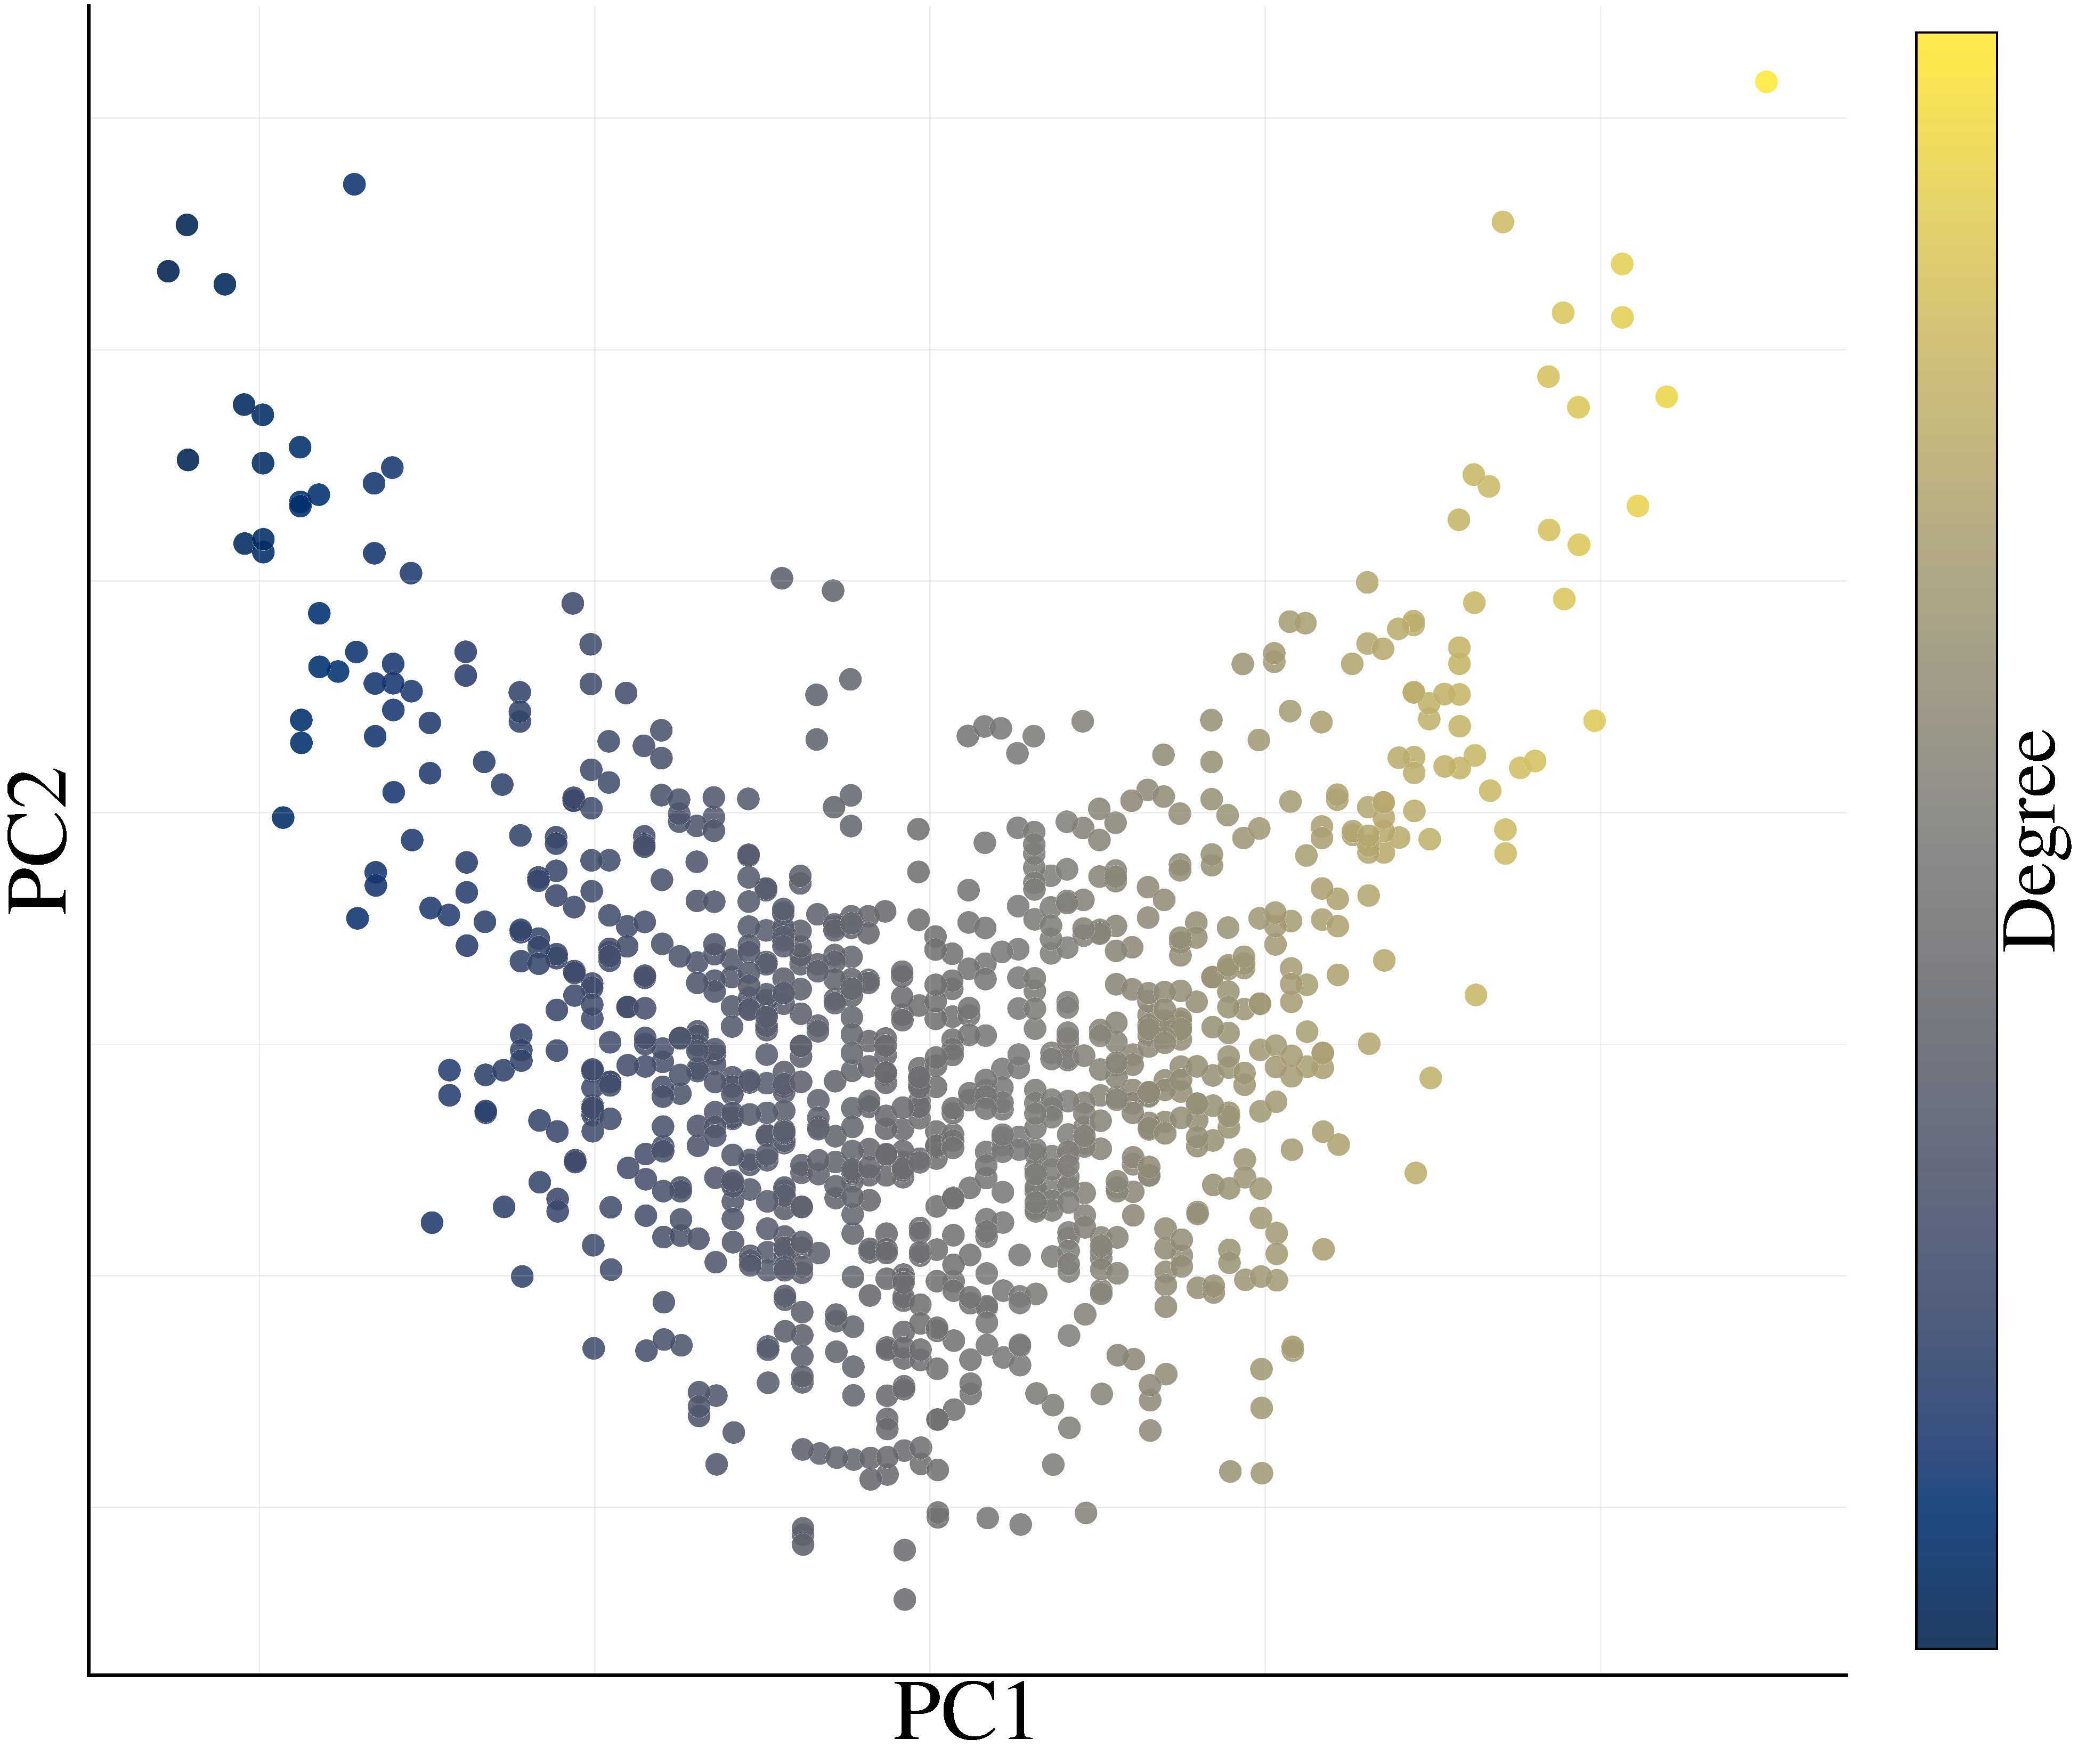
\includegraphics[width=\linewidth]{SGNN_objective_train_medium_g0_pc1_pc2_degree.pdf}
    \smallskip
    \textbf{(a)} \textsc{SGNN}.
  \end{minipage}\hfill
  \begin{minipage}{0.45\textwidth}
    \centering
    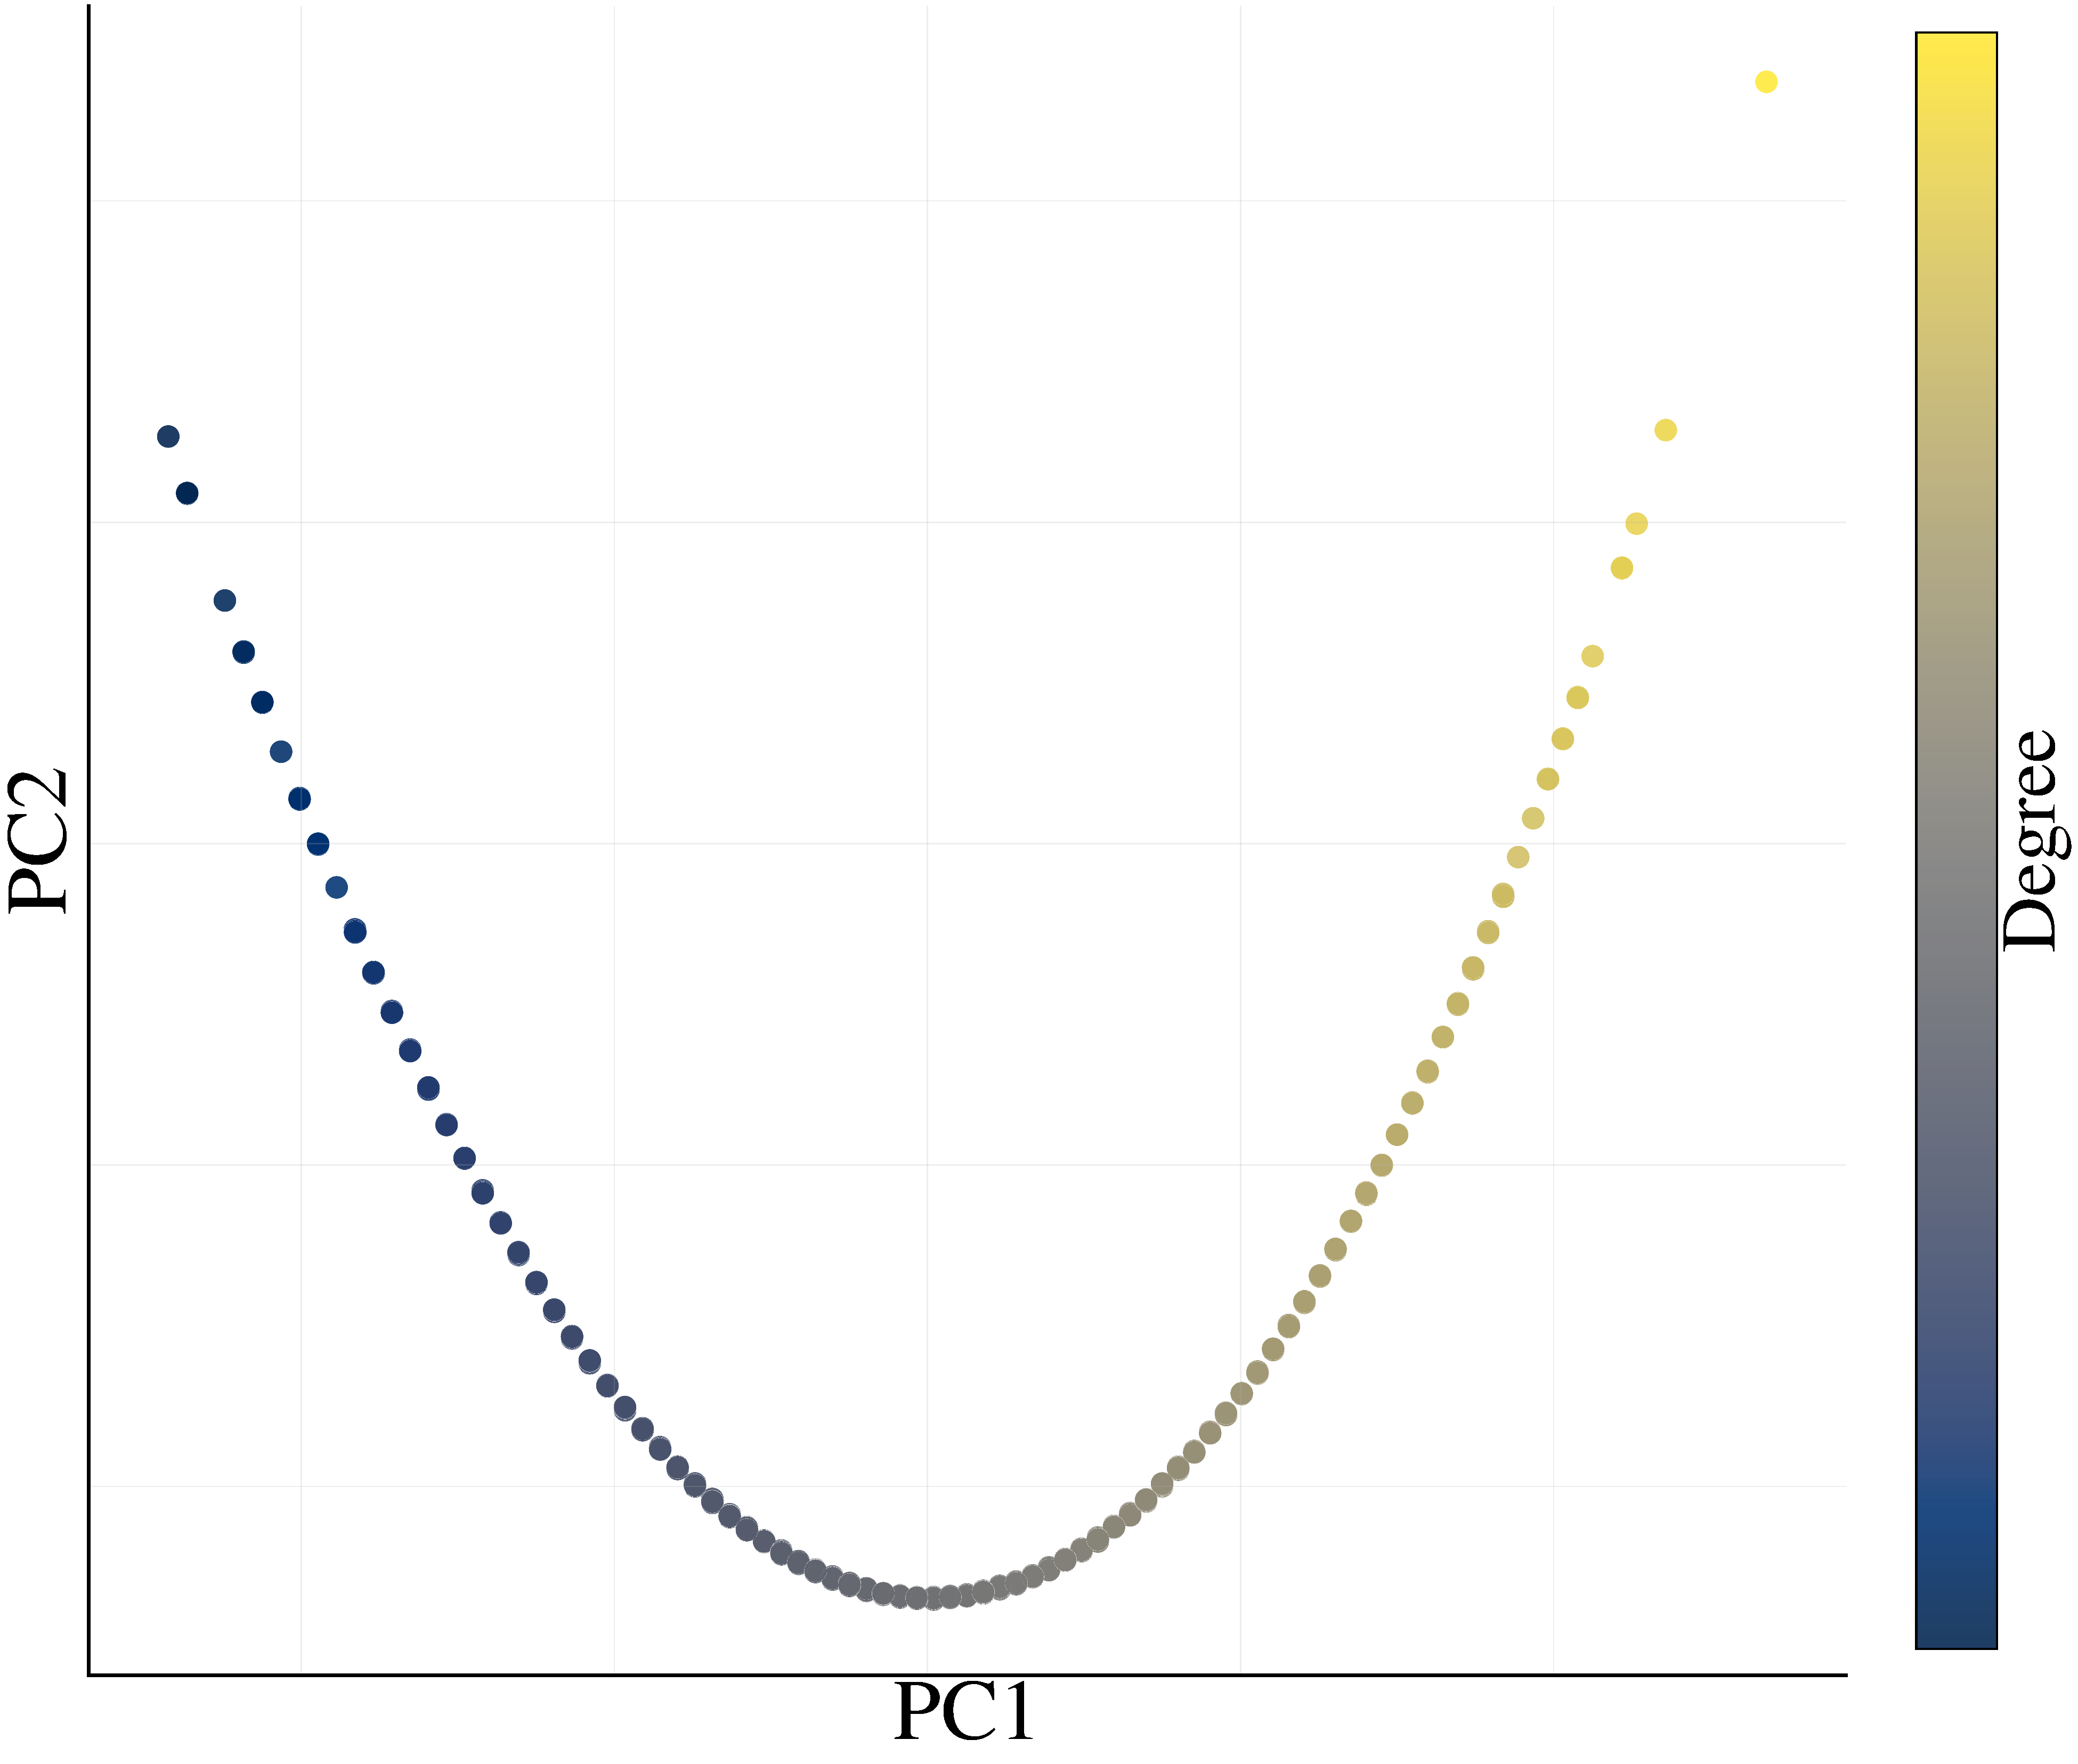
\includegraphics[width=\linewidth]{SGNN_U_self_predictor_lpr_train_medium_g0_pc1_pc2_degree.pdf}
    \smallskip
    \textbf{(b)} \textsc{SGNN+U}.
  \end{minipage}\hfill
  \begin{minipage}{0.45\textwidth}
    \centering
    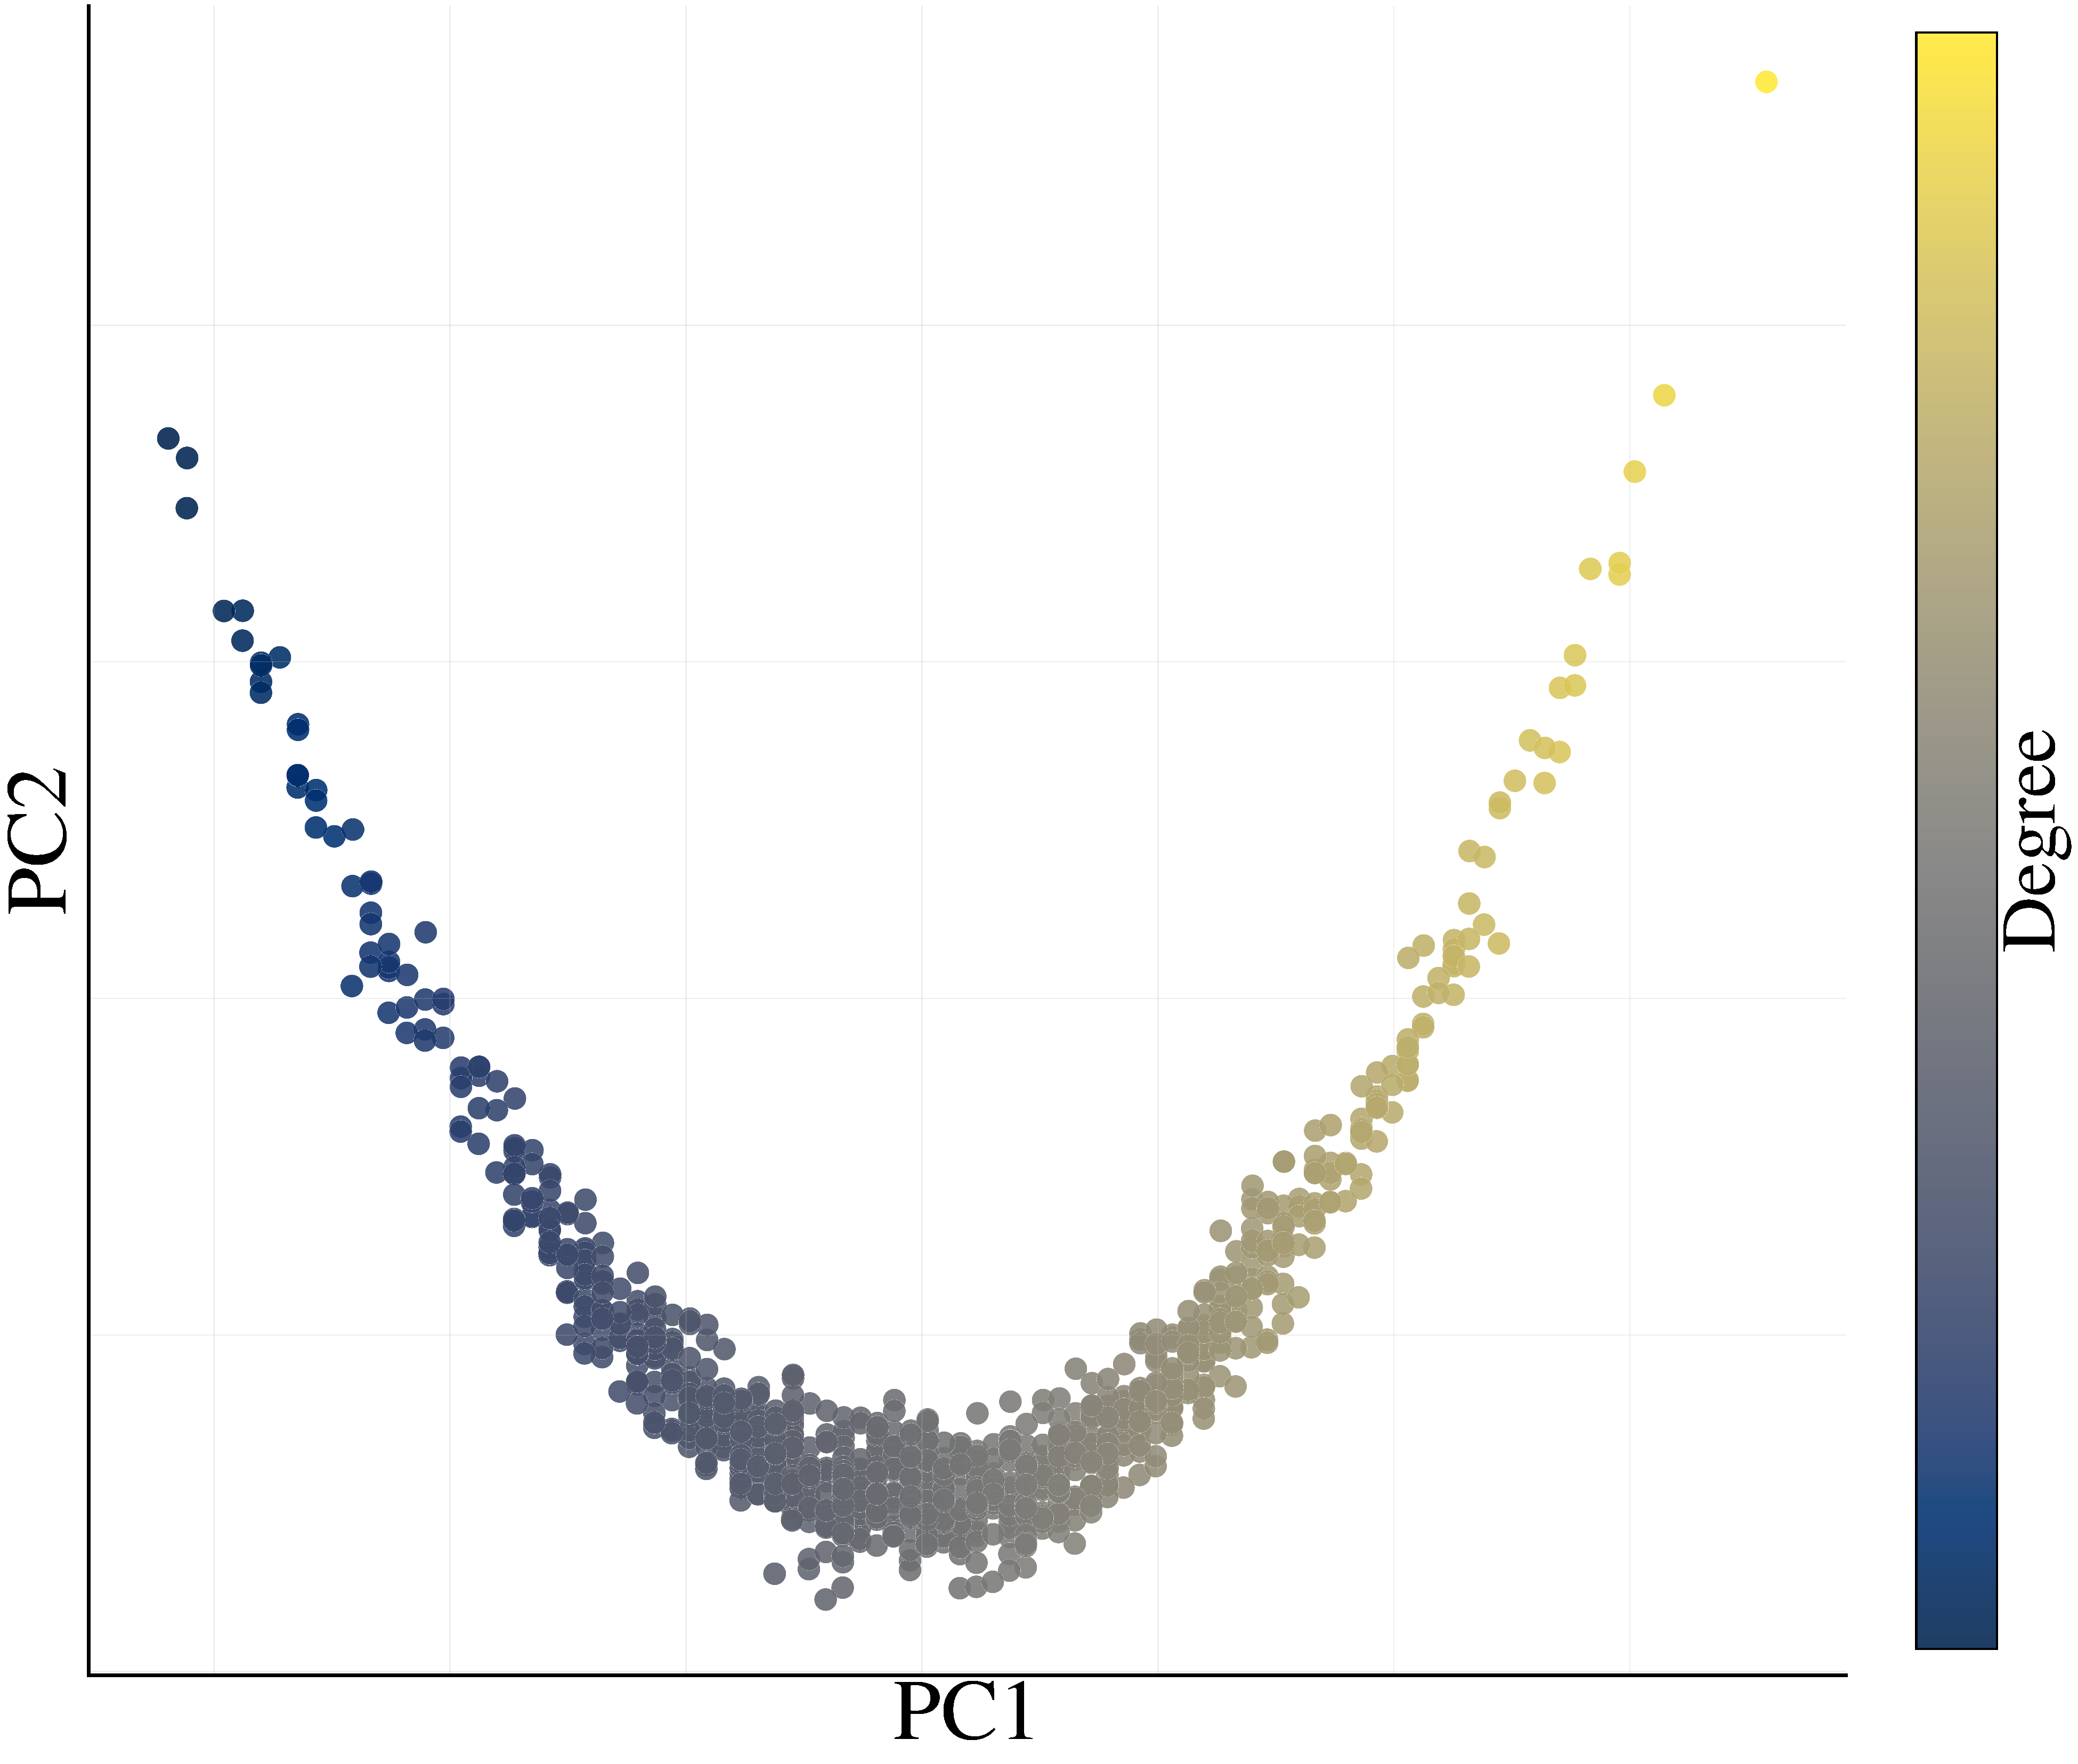
\includegraphics[width=\linewidth]{SGNN_GU_self_predictor_lpr_train_medium_g0_pc1_pc2_degree.pdf}
    \smallskip
    \textbf{(c)} \textsc{SGNN+GU}.
  \end{minipage}
  \caption{Final-layer representation geometry. (\textbf{a}) \textsc{SGNN},
    (\textbf{b}) \textsc{SGNN+U}, and (\textbf{c}) \textsc{SGNN+GU}: vertices plotted
    in the first two principal-component coordinates of the last GNN layer,
    color-coded by residual degree. Across all three panels, the colors are ordered
    almost entirely along PC1, indicating that the final GNN embedding has collapsed
  to a one-dimensional degree axis; PC2 adds little visible structure.}
  \label{fig:pca_degree_embeddings}
\end{figure}

\subsubsection{The Updater Exhibits Low-Degree Pruning Behavior}

After one application of $U_\theta$, the absolute Spearman correlation between
residual degree and updated scores drops to $0.36$--$0.52$, so the successful
updater is not merely preserving the raw degree ranking. The relevant signal is
coarser and more operational: whether the updater prevents U-LPR from deleting
vertices whose residual degree is too high. \textsc{SGNN+U} removes an
at-or-below-15th-percentile-degree vertex on only $14.7\%$ of U-LPR steps---a rate
consistent with random vertex selection---while \textsc{SGNN+GU} does so on $100.0\%$
of steps.

Table~\ref{tab:percentile} extends this diagnostic across multiple percentile
thresholds $\tau$. \textsc{SGNN+GU} maintains near-$100\%$ below-threshold deletions
at every value of $\tau$ tested, whereas the \textsc{SGNN+U} rate tracks $\tau$
itself, confirming random behavior. The qualitative separation is robust across all
thresholds tested; the 15th percentile is used as the primary threshold in
Table~\ref{tab:pca} because it is the lowest value at which \textsc{SGNN+GU}
maintains near-zero above-threshold deletions.

\begin{table}[H]
  \caption{Fraction of U-LPR deletion steps in which the removed vertex falls
    \emph{at or below} residual-degree percentile threshold $\tau$, measured on
    the Medium regime over 1000 graphs. Rows are shown for thresholds with exact
    measurements; tests at $\tau\in\{10,30\}$ yield \textsc{SGNN+GU} values
    $\geq99.9\%$ and \textsc{SGNN+U} values within $1\%$ of $\tau$, consistent
  with the pattern below.}
  \label{tab:percentile}
  \centering
  \begin{tabular}{ccc}
    \toprule
    $\tau$ (\%) & \textsc{SGNN+GU} mean$\pm$std & \textsc{SGNN+U} mean$\pm$std \\
    \midrule
    50 & $100.0\pm 0.0$ & $50.1\pm 2.5$ \\
    30 & $100.0\pm 0.0$ & $29.3\pm 1.8$ \\
    15 & $100.0\pm 0.0$ & $14.7\pm 1.3$ \\
    10 & $99.0\pm 0.01$ & $10.1\pm 0.9$ \\
    \bottomrule
  \end{tabular}
\end{table}

Thus the diagnostic supports a coarse low-degree pruning behavior, rather than an
exact degree sort or a formally extracted internal concept. In our experiments, the
gradient channel makes this behavior reliable throughout the residual loop by
exposing the local change in the objective after each deletion. In
Figure~\ref{fig:score_degree_pruning_grid}, we see score--degree scatter plots
arranged with pruning iterations as rows and model variants as columns; the marked
deletion stays below the 15th-percentile line for \textsc{SGNN+GU} but not for
\textsc{SGNN+U}.

\begin{figure}[H]
  \centering
  \begin{adjustbox}{max width=\textwidth}
    \begin{tabular}{@{}c c c@{}}
      & \textsc{SGNN+U} & \textsc{SGNN+GU} \\
      \raisebox{-.5\height}{$t=0$}
      & \raisebox{-.5\height}{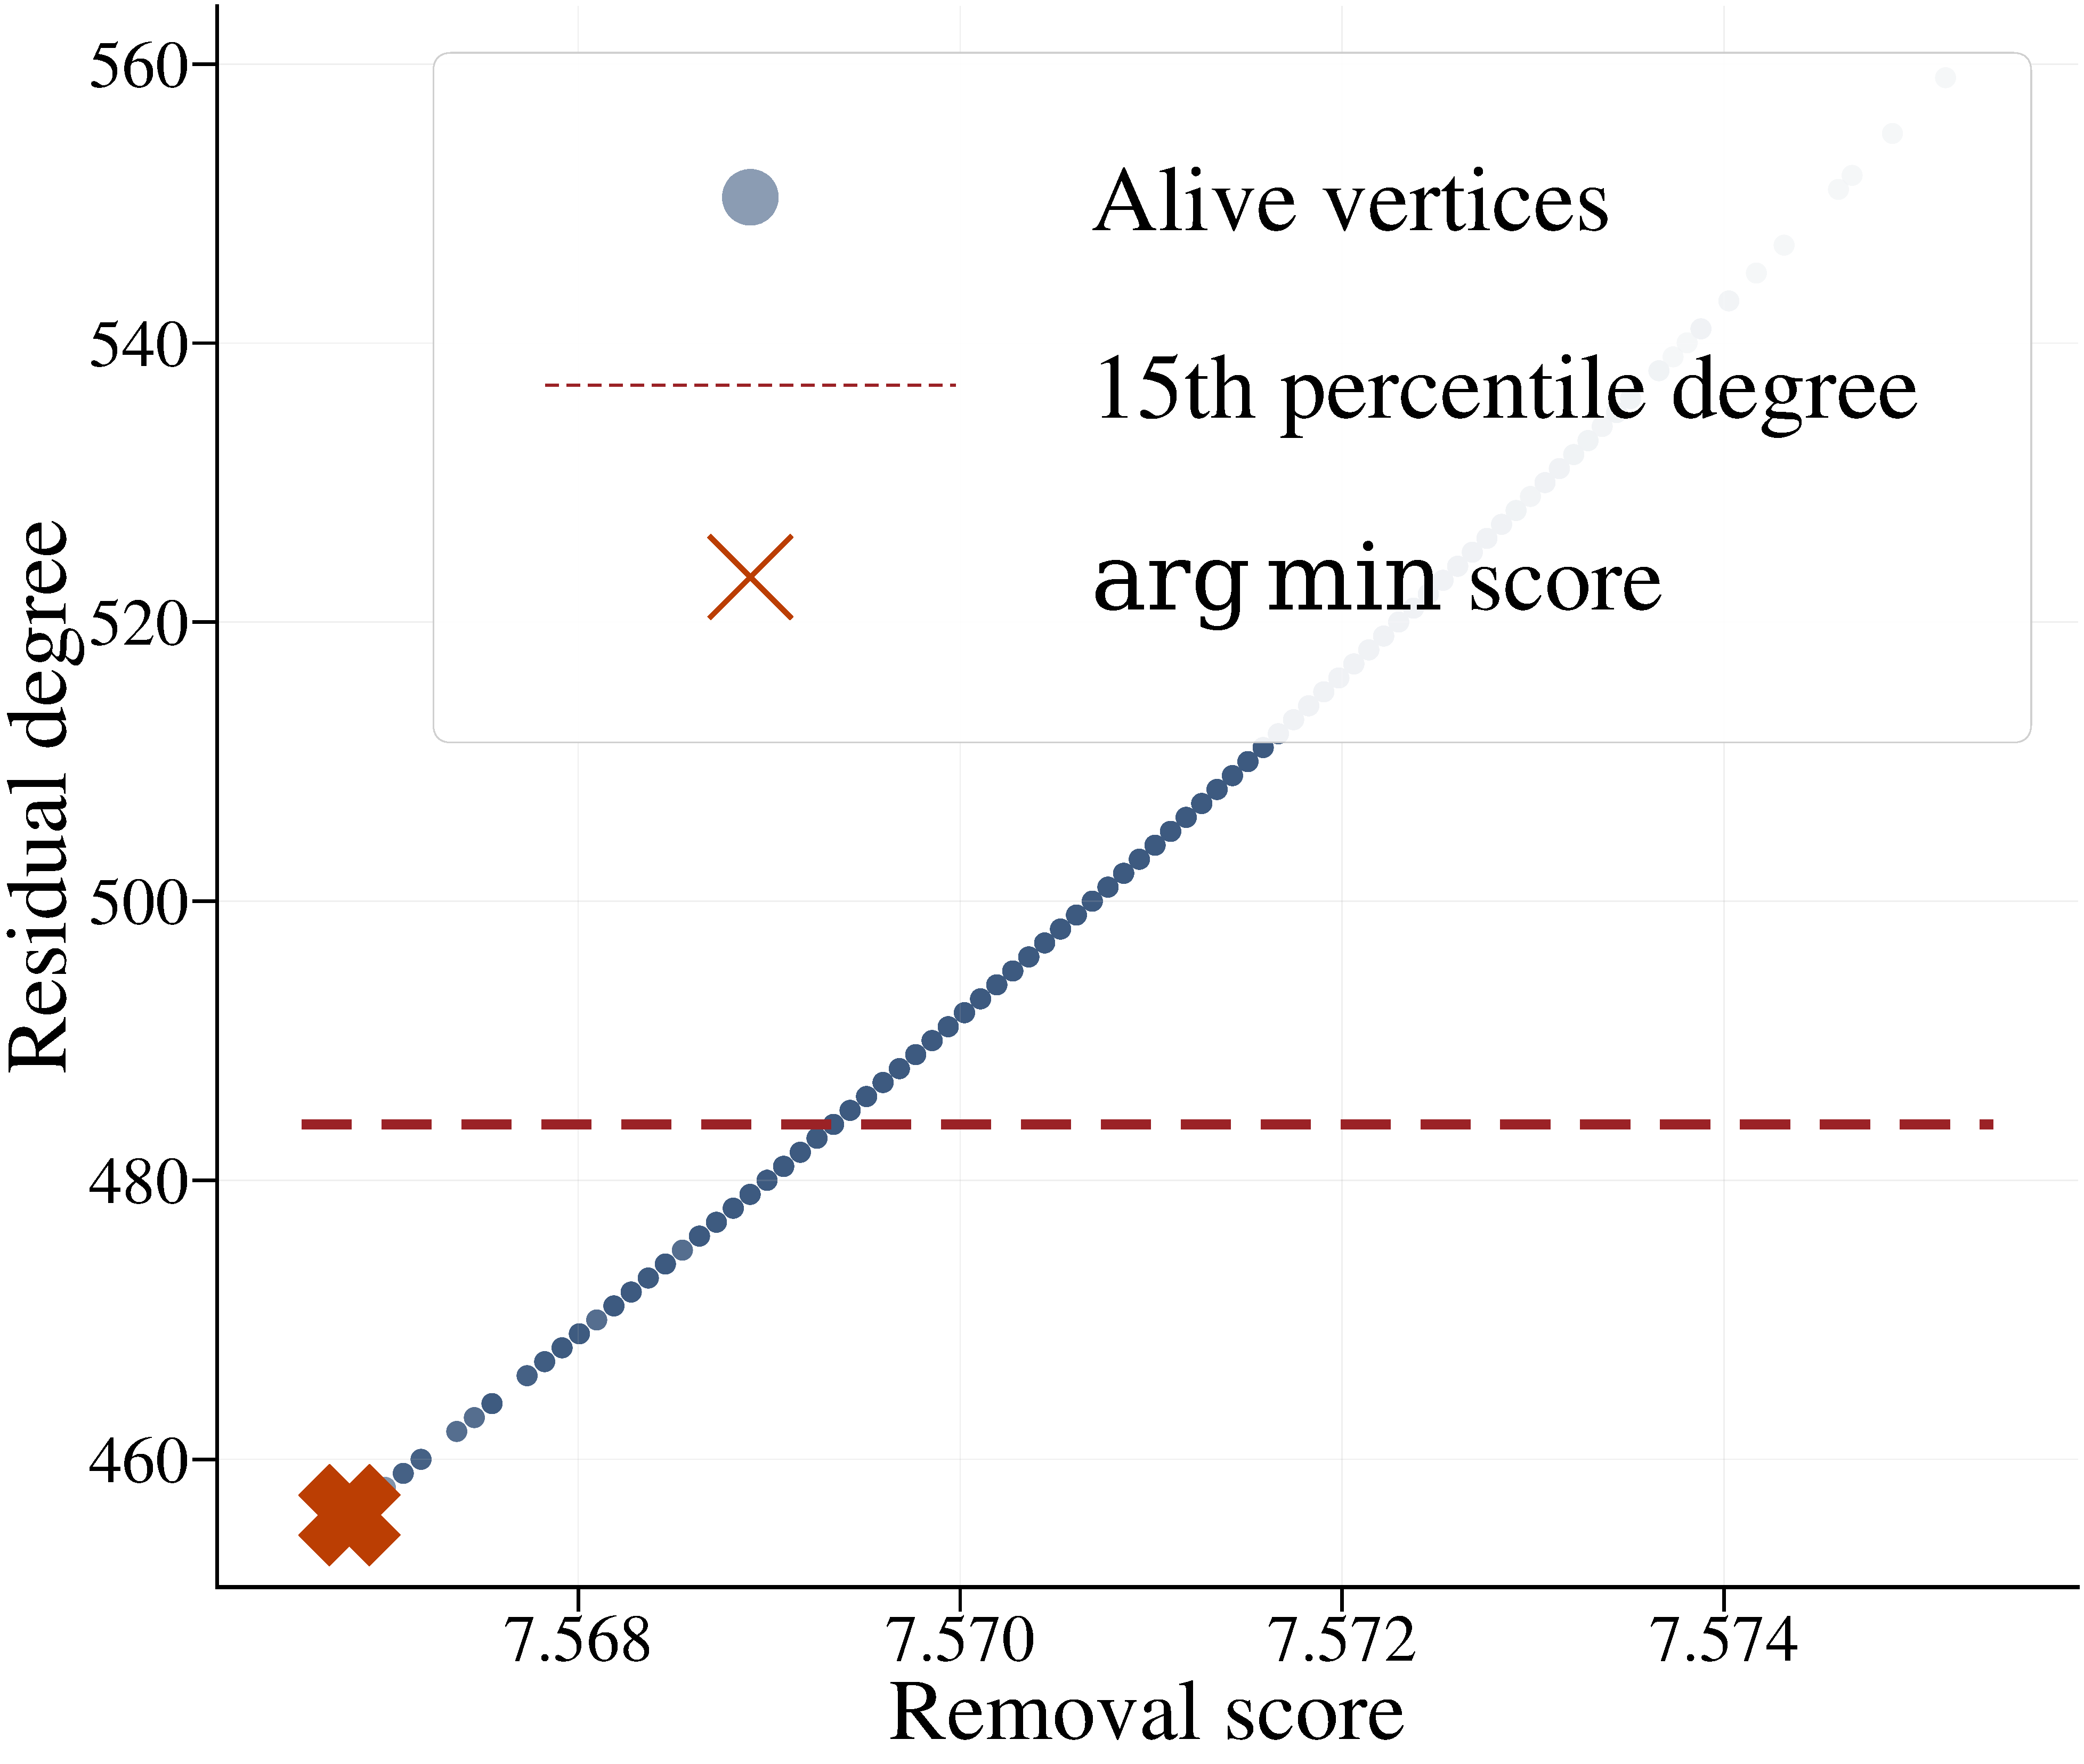
\includegraphics[width=0.38\textwidth]{SGNN_U_self_predictor_lpr_train_medium_g0_upr_step0_score_vs_degree.pdf}}
      & \raisebox{-.5\height}{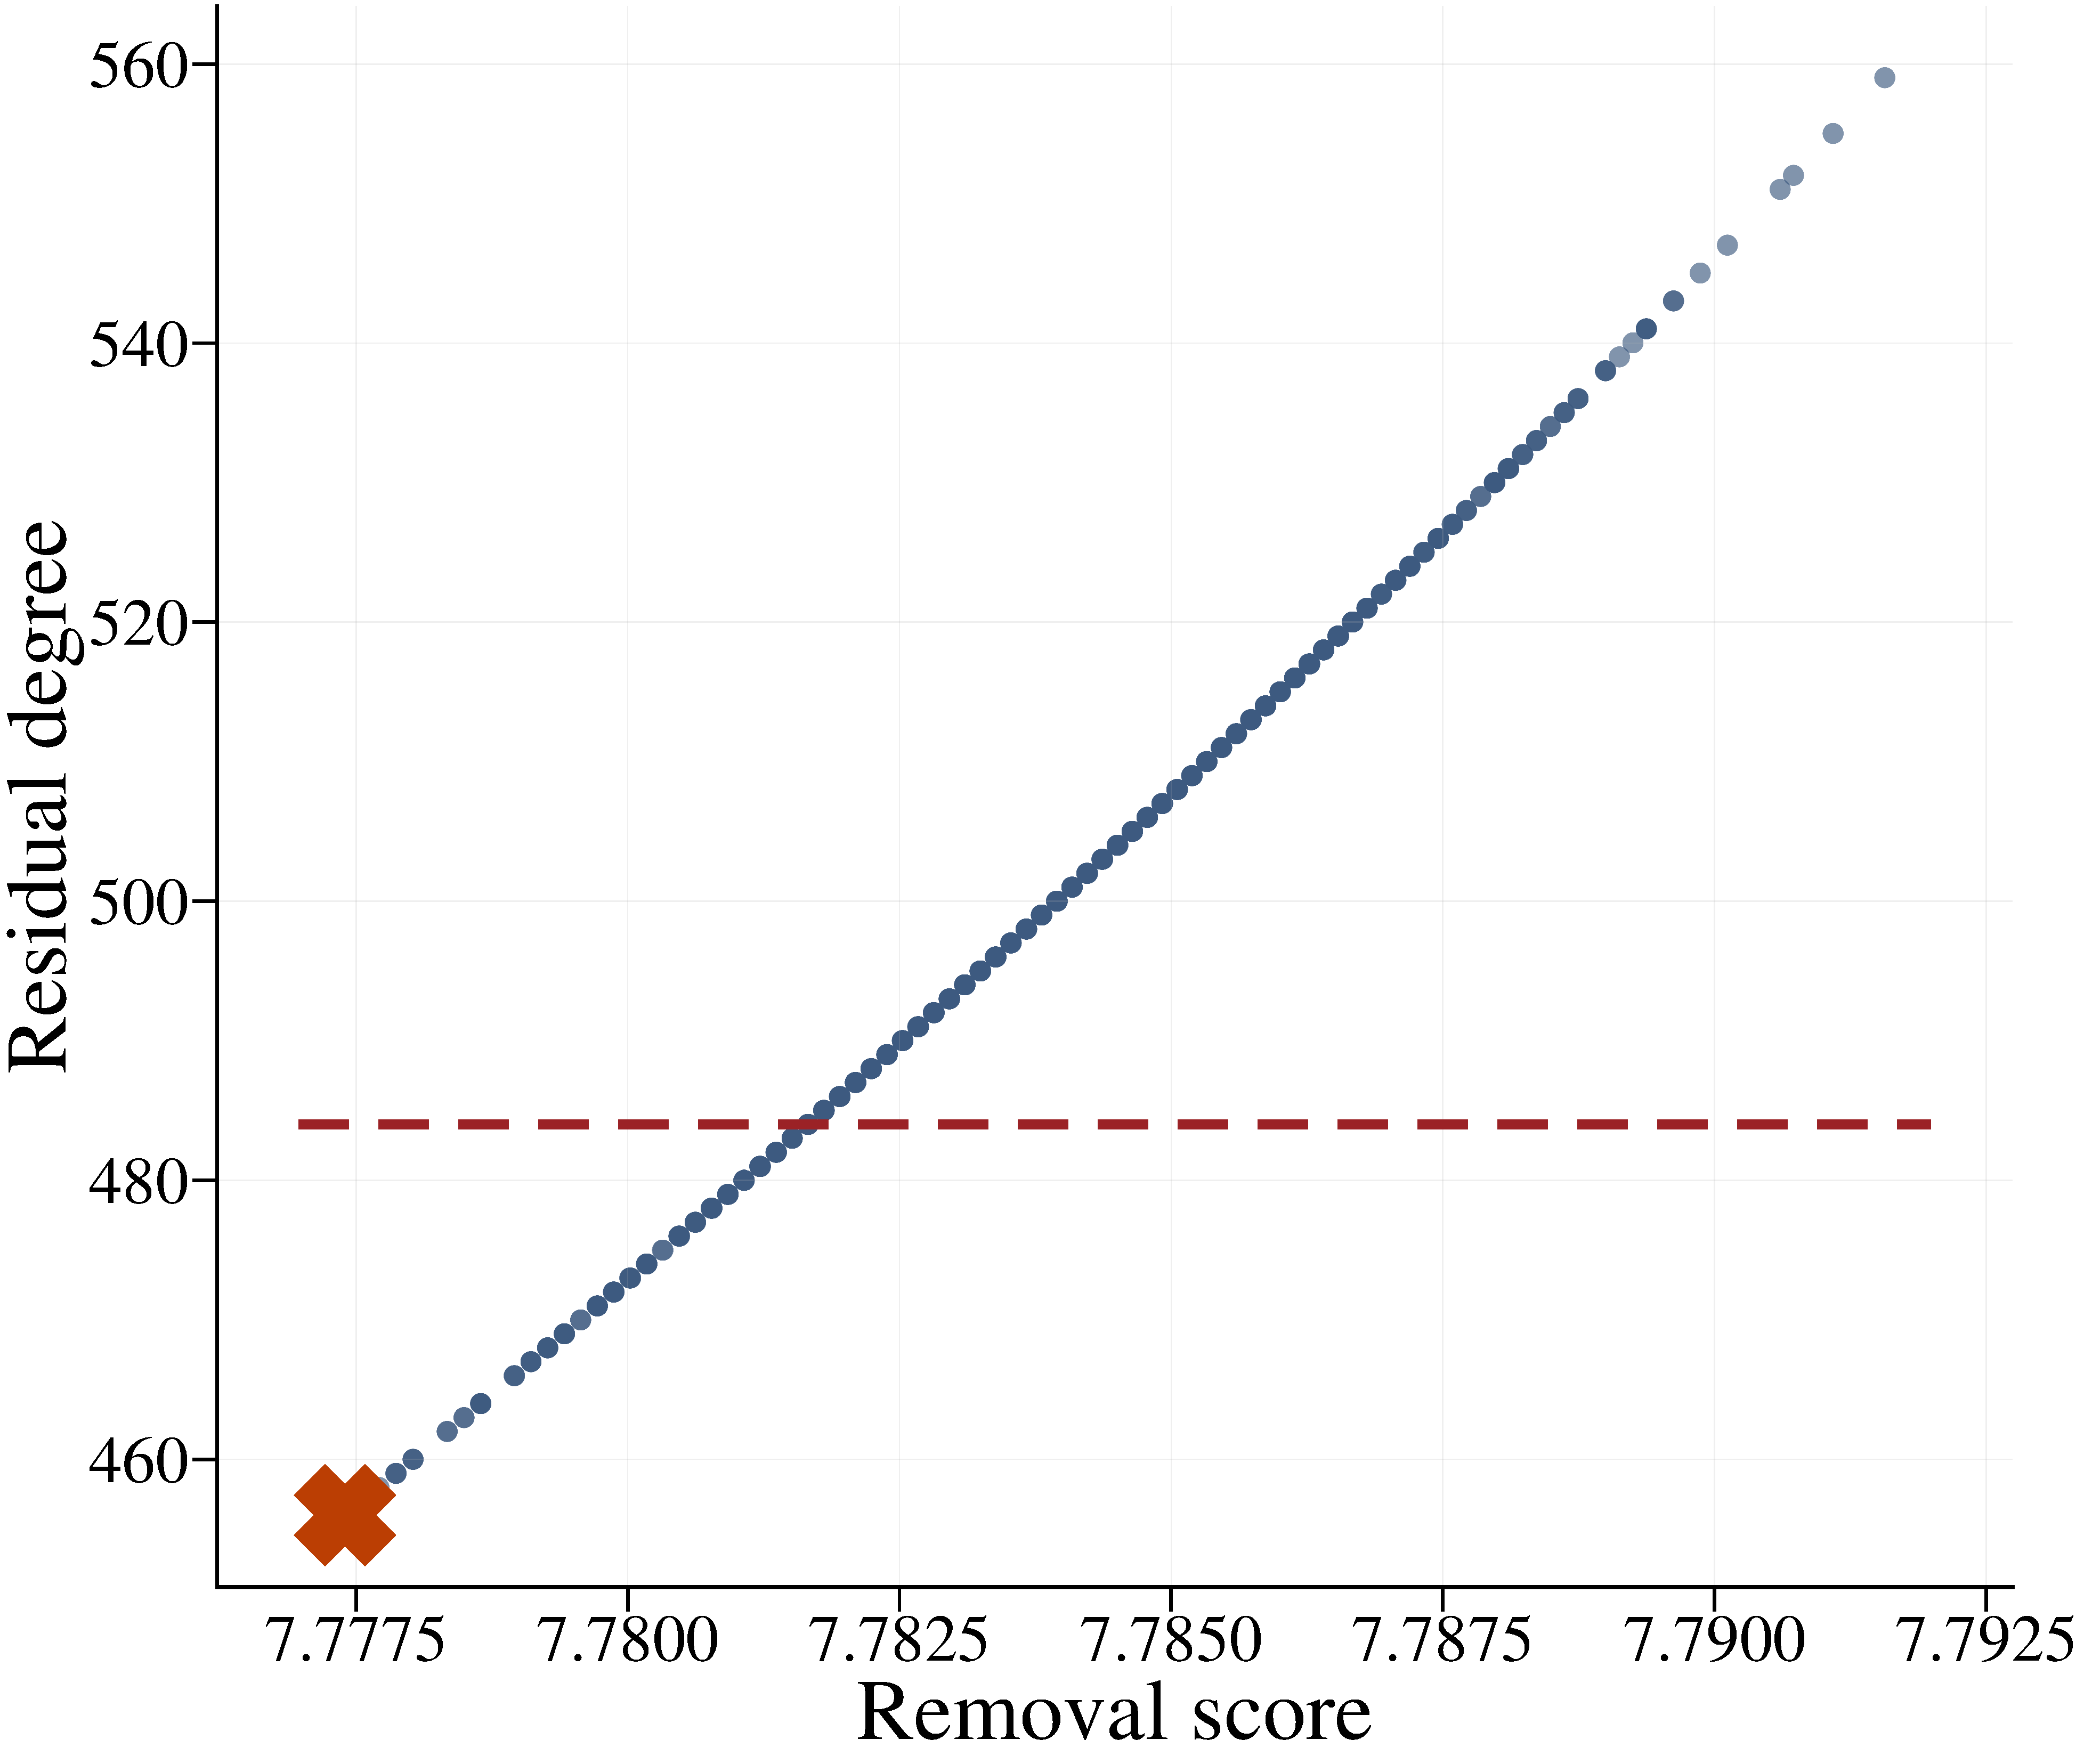
\includegraphics[width=0.38\textwidth]{SGNN_GU_self_predictor_lpr_train_medium_g0_upr_step0_score_vs_degree.pdf}} \\
      \raisebox{-.5\height}{$t=5$}
      & \raisebox{-.5\height}{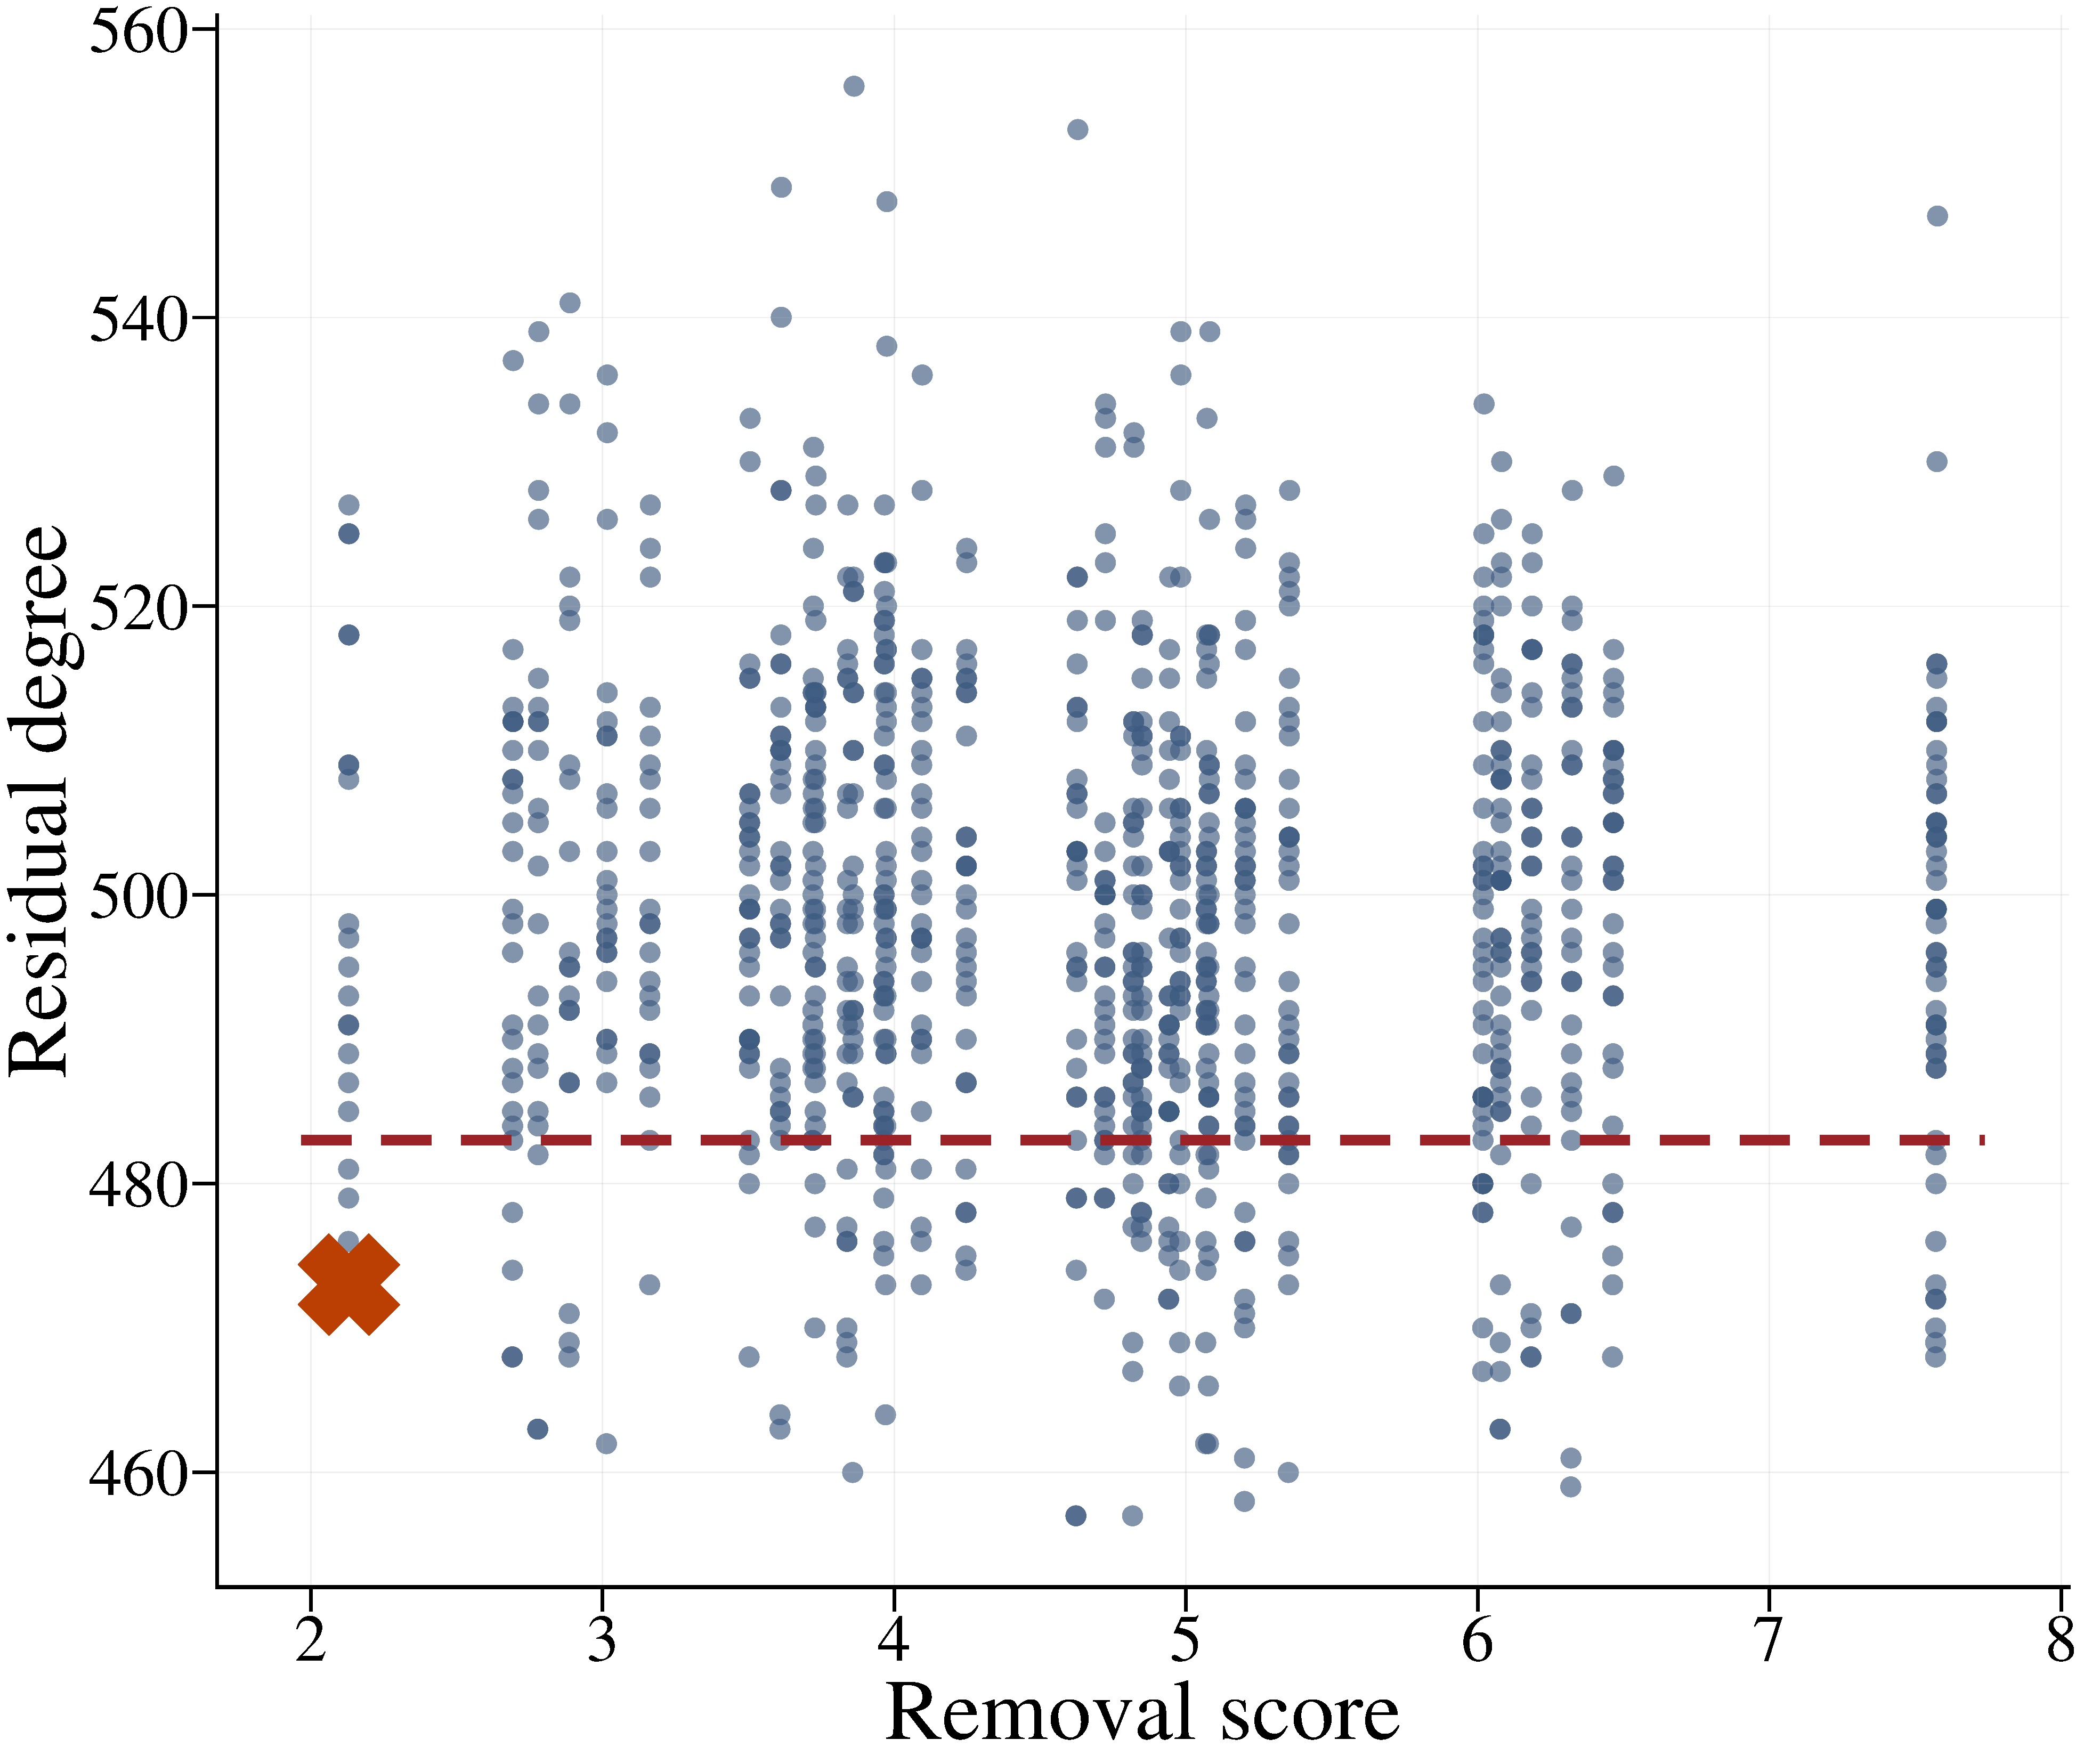
\includegraphics[width=0.38\textwidth]{SGNN_U_self_predictor_lpr_train_medium_g0_upr_step5_score_vs_degree.pdf}}
      & \raisebox{-.5\height}{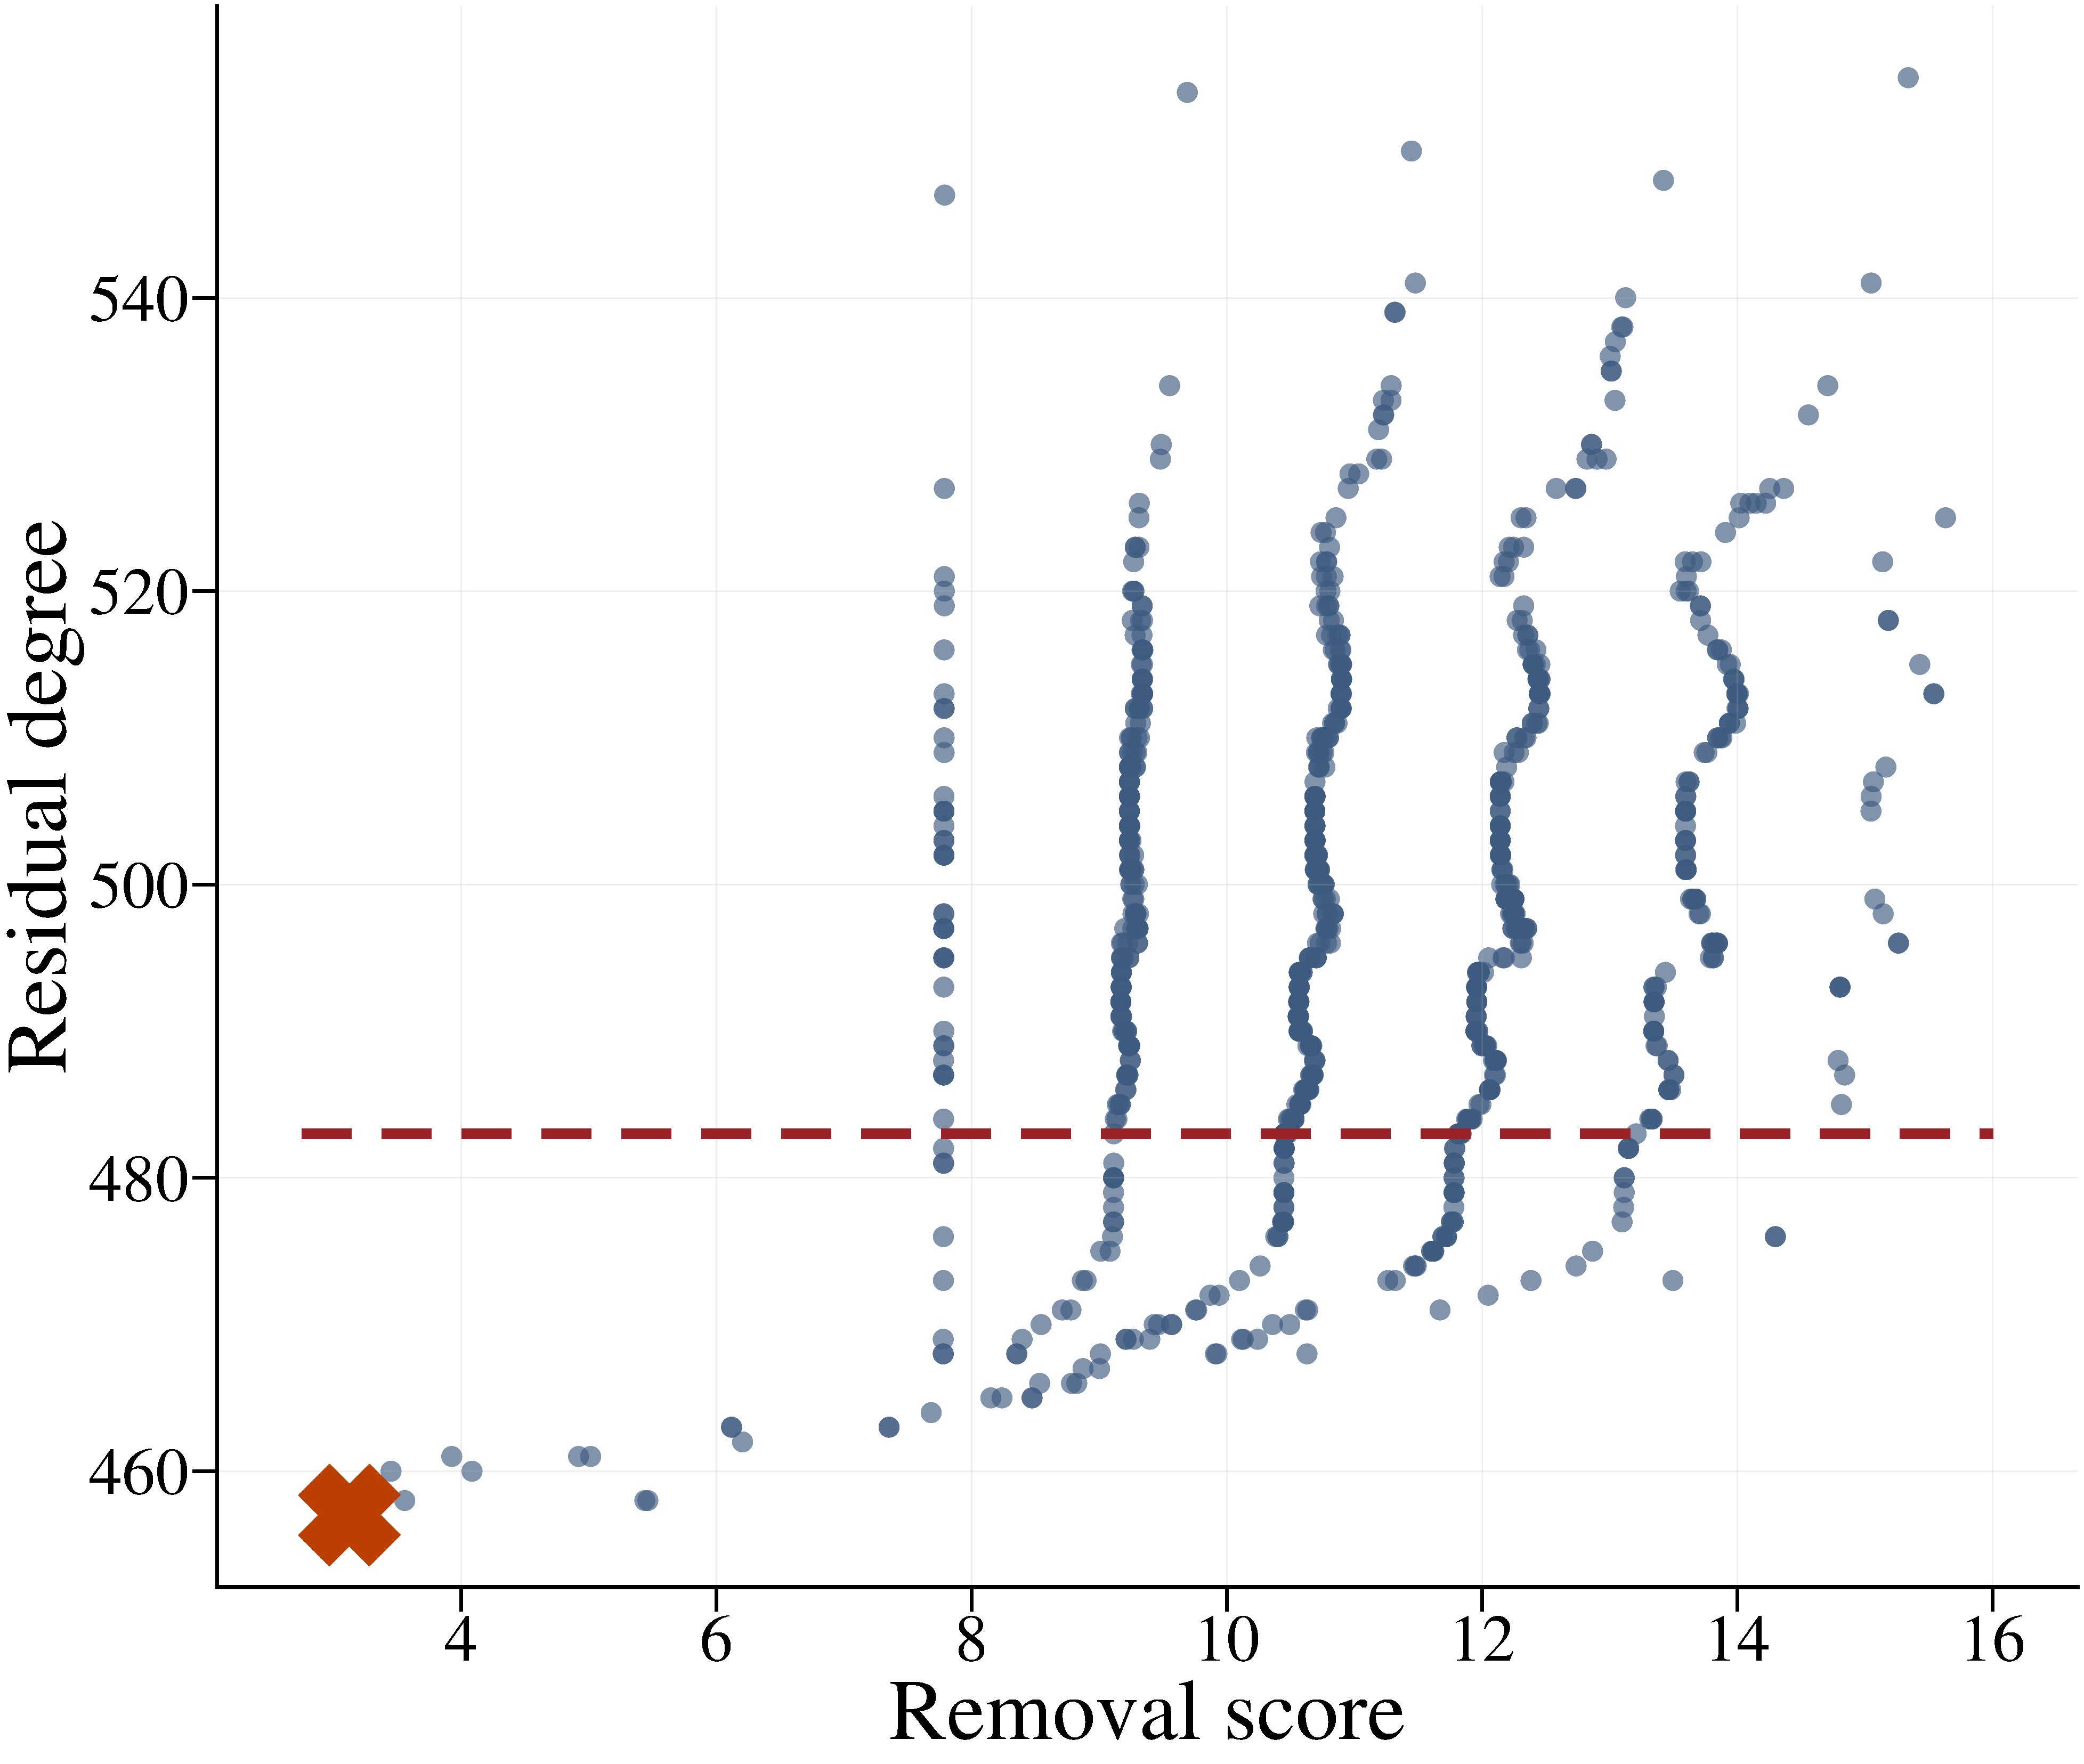
\includegraphics[width=0.38\textwidth]{SGNN_GU_self_predictor_lpr_train_medium_g0_upr_step5_score_vs_degree.pdf}} \\
      \raisebox{-.5\height}{$t=300$}
      & \raisebox{-.5\height}{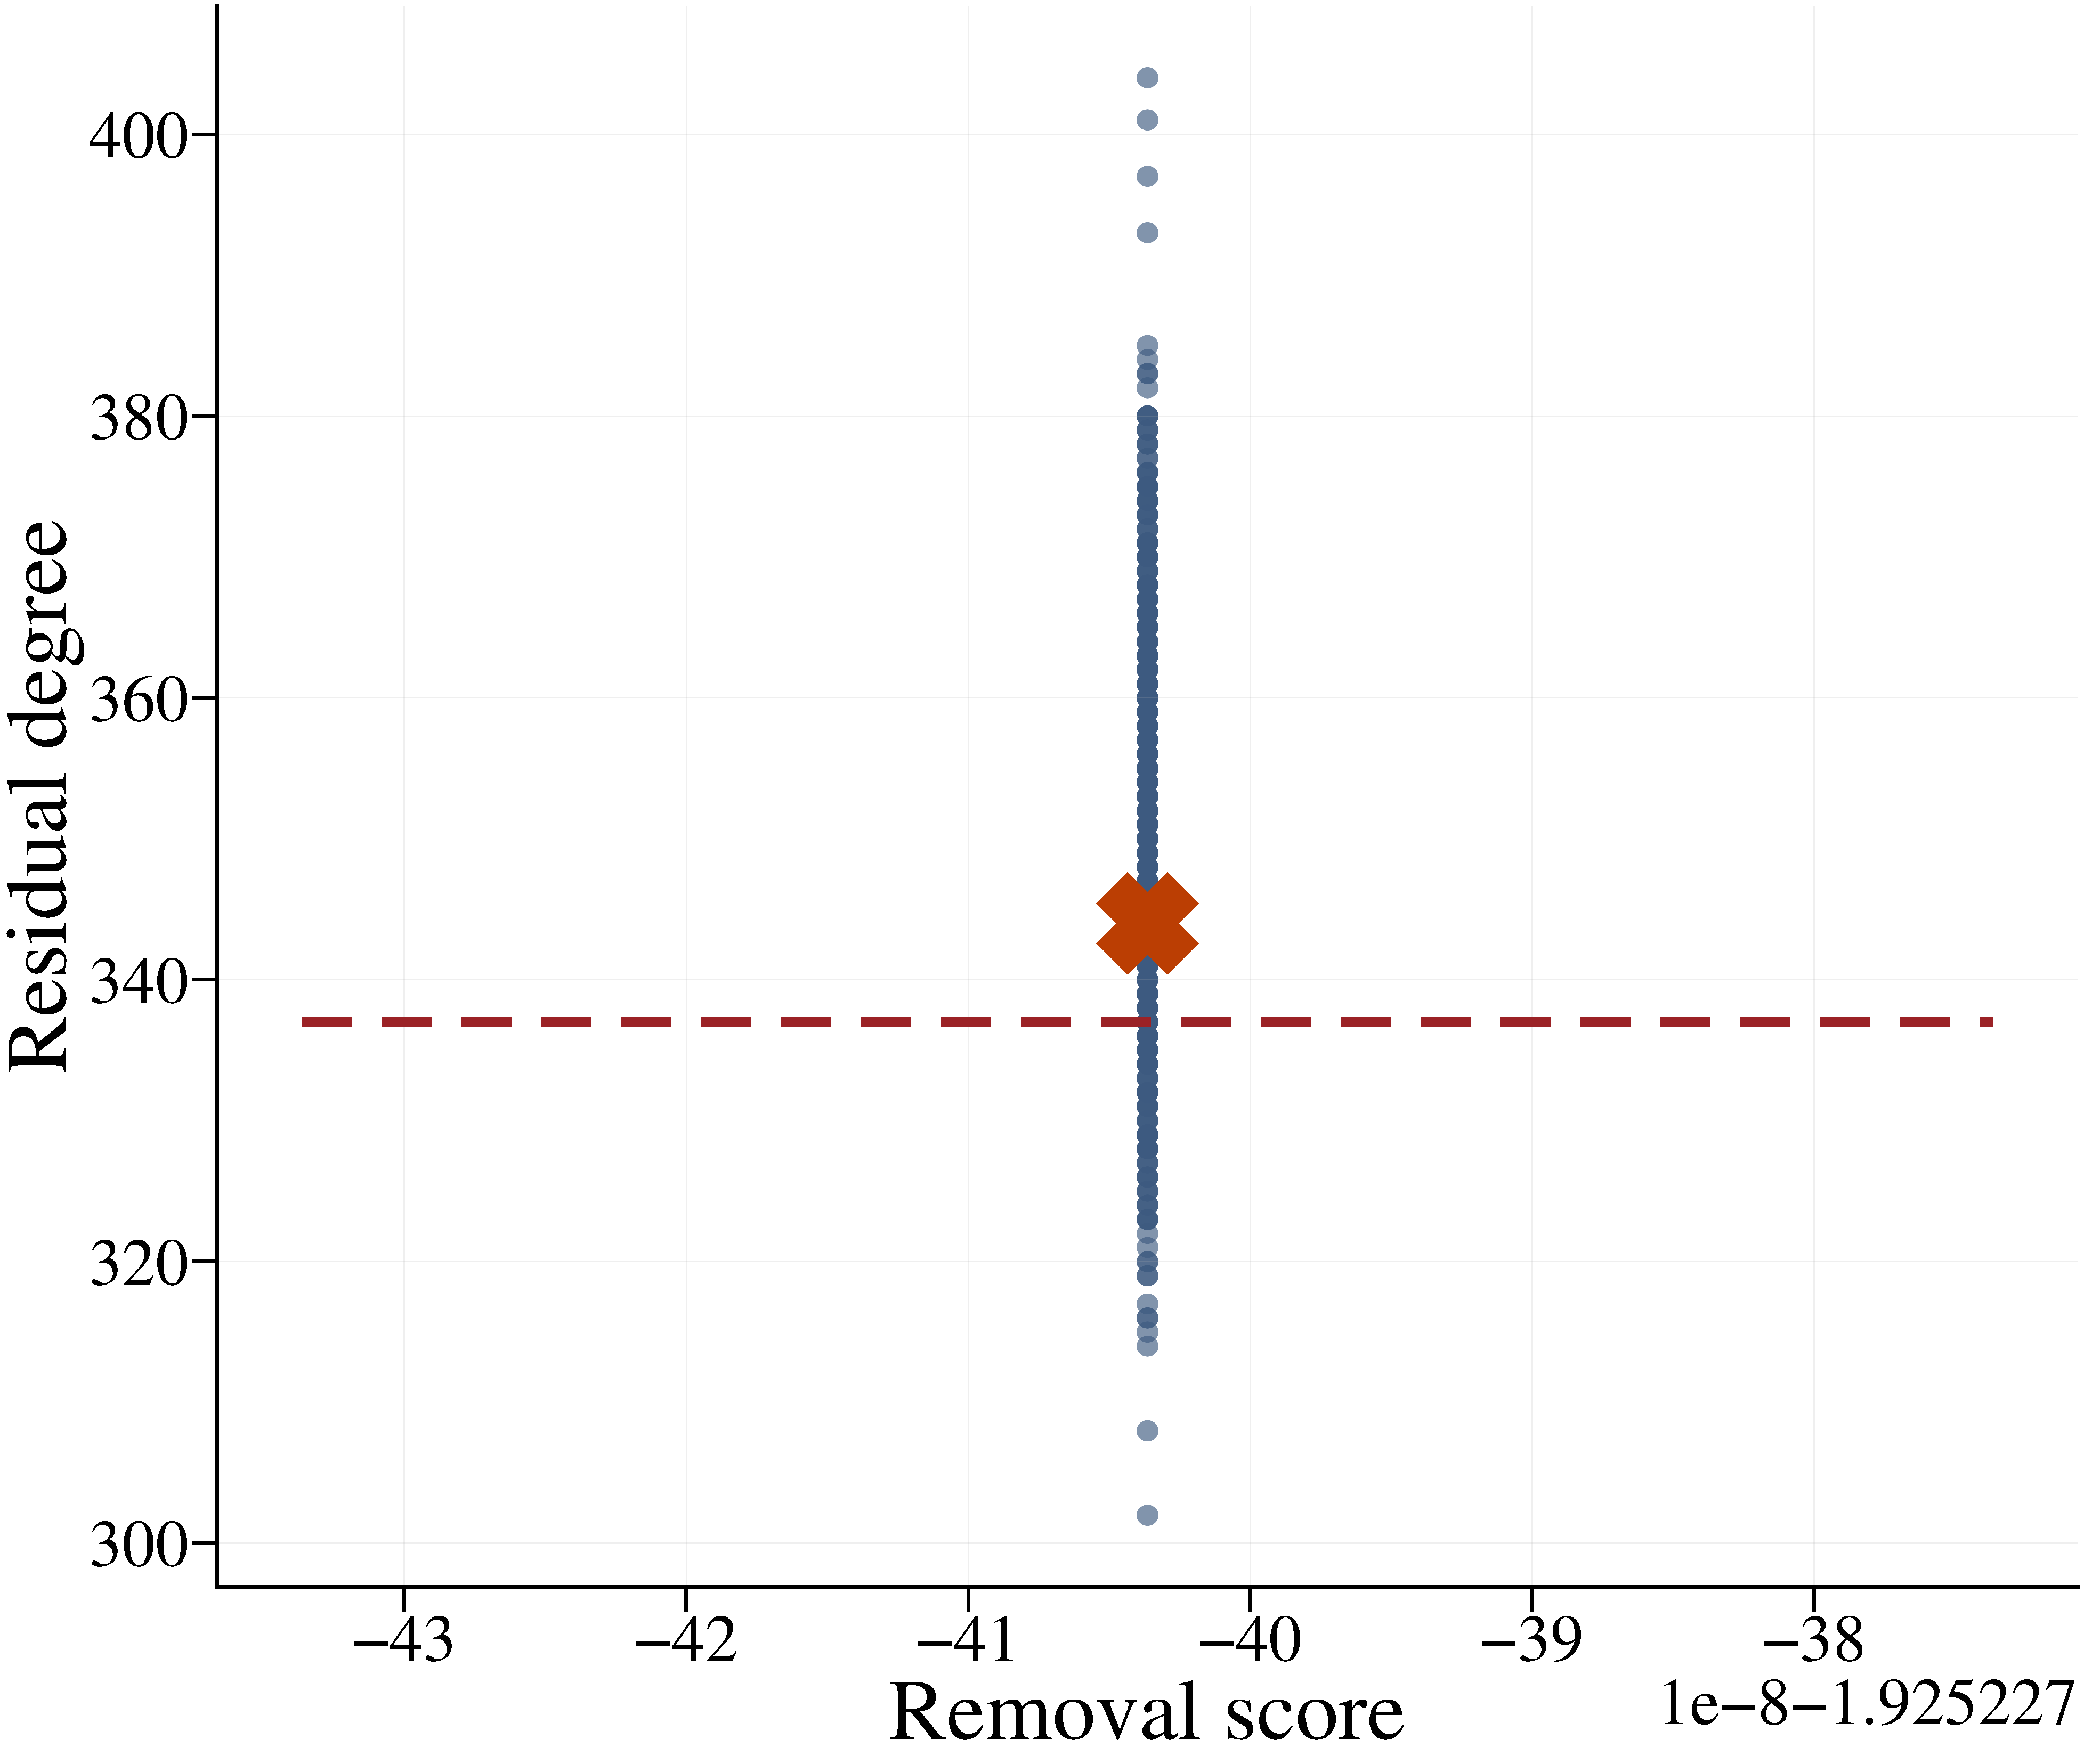
\includegraphics[width=0.38\textwidth]{SGNN_U_self_predictor_lpr_train_medium_g0_upr_step300_score_vs_degree.pdf}}
      & \raisebox{-.5\height}{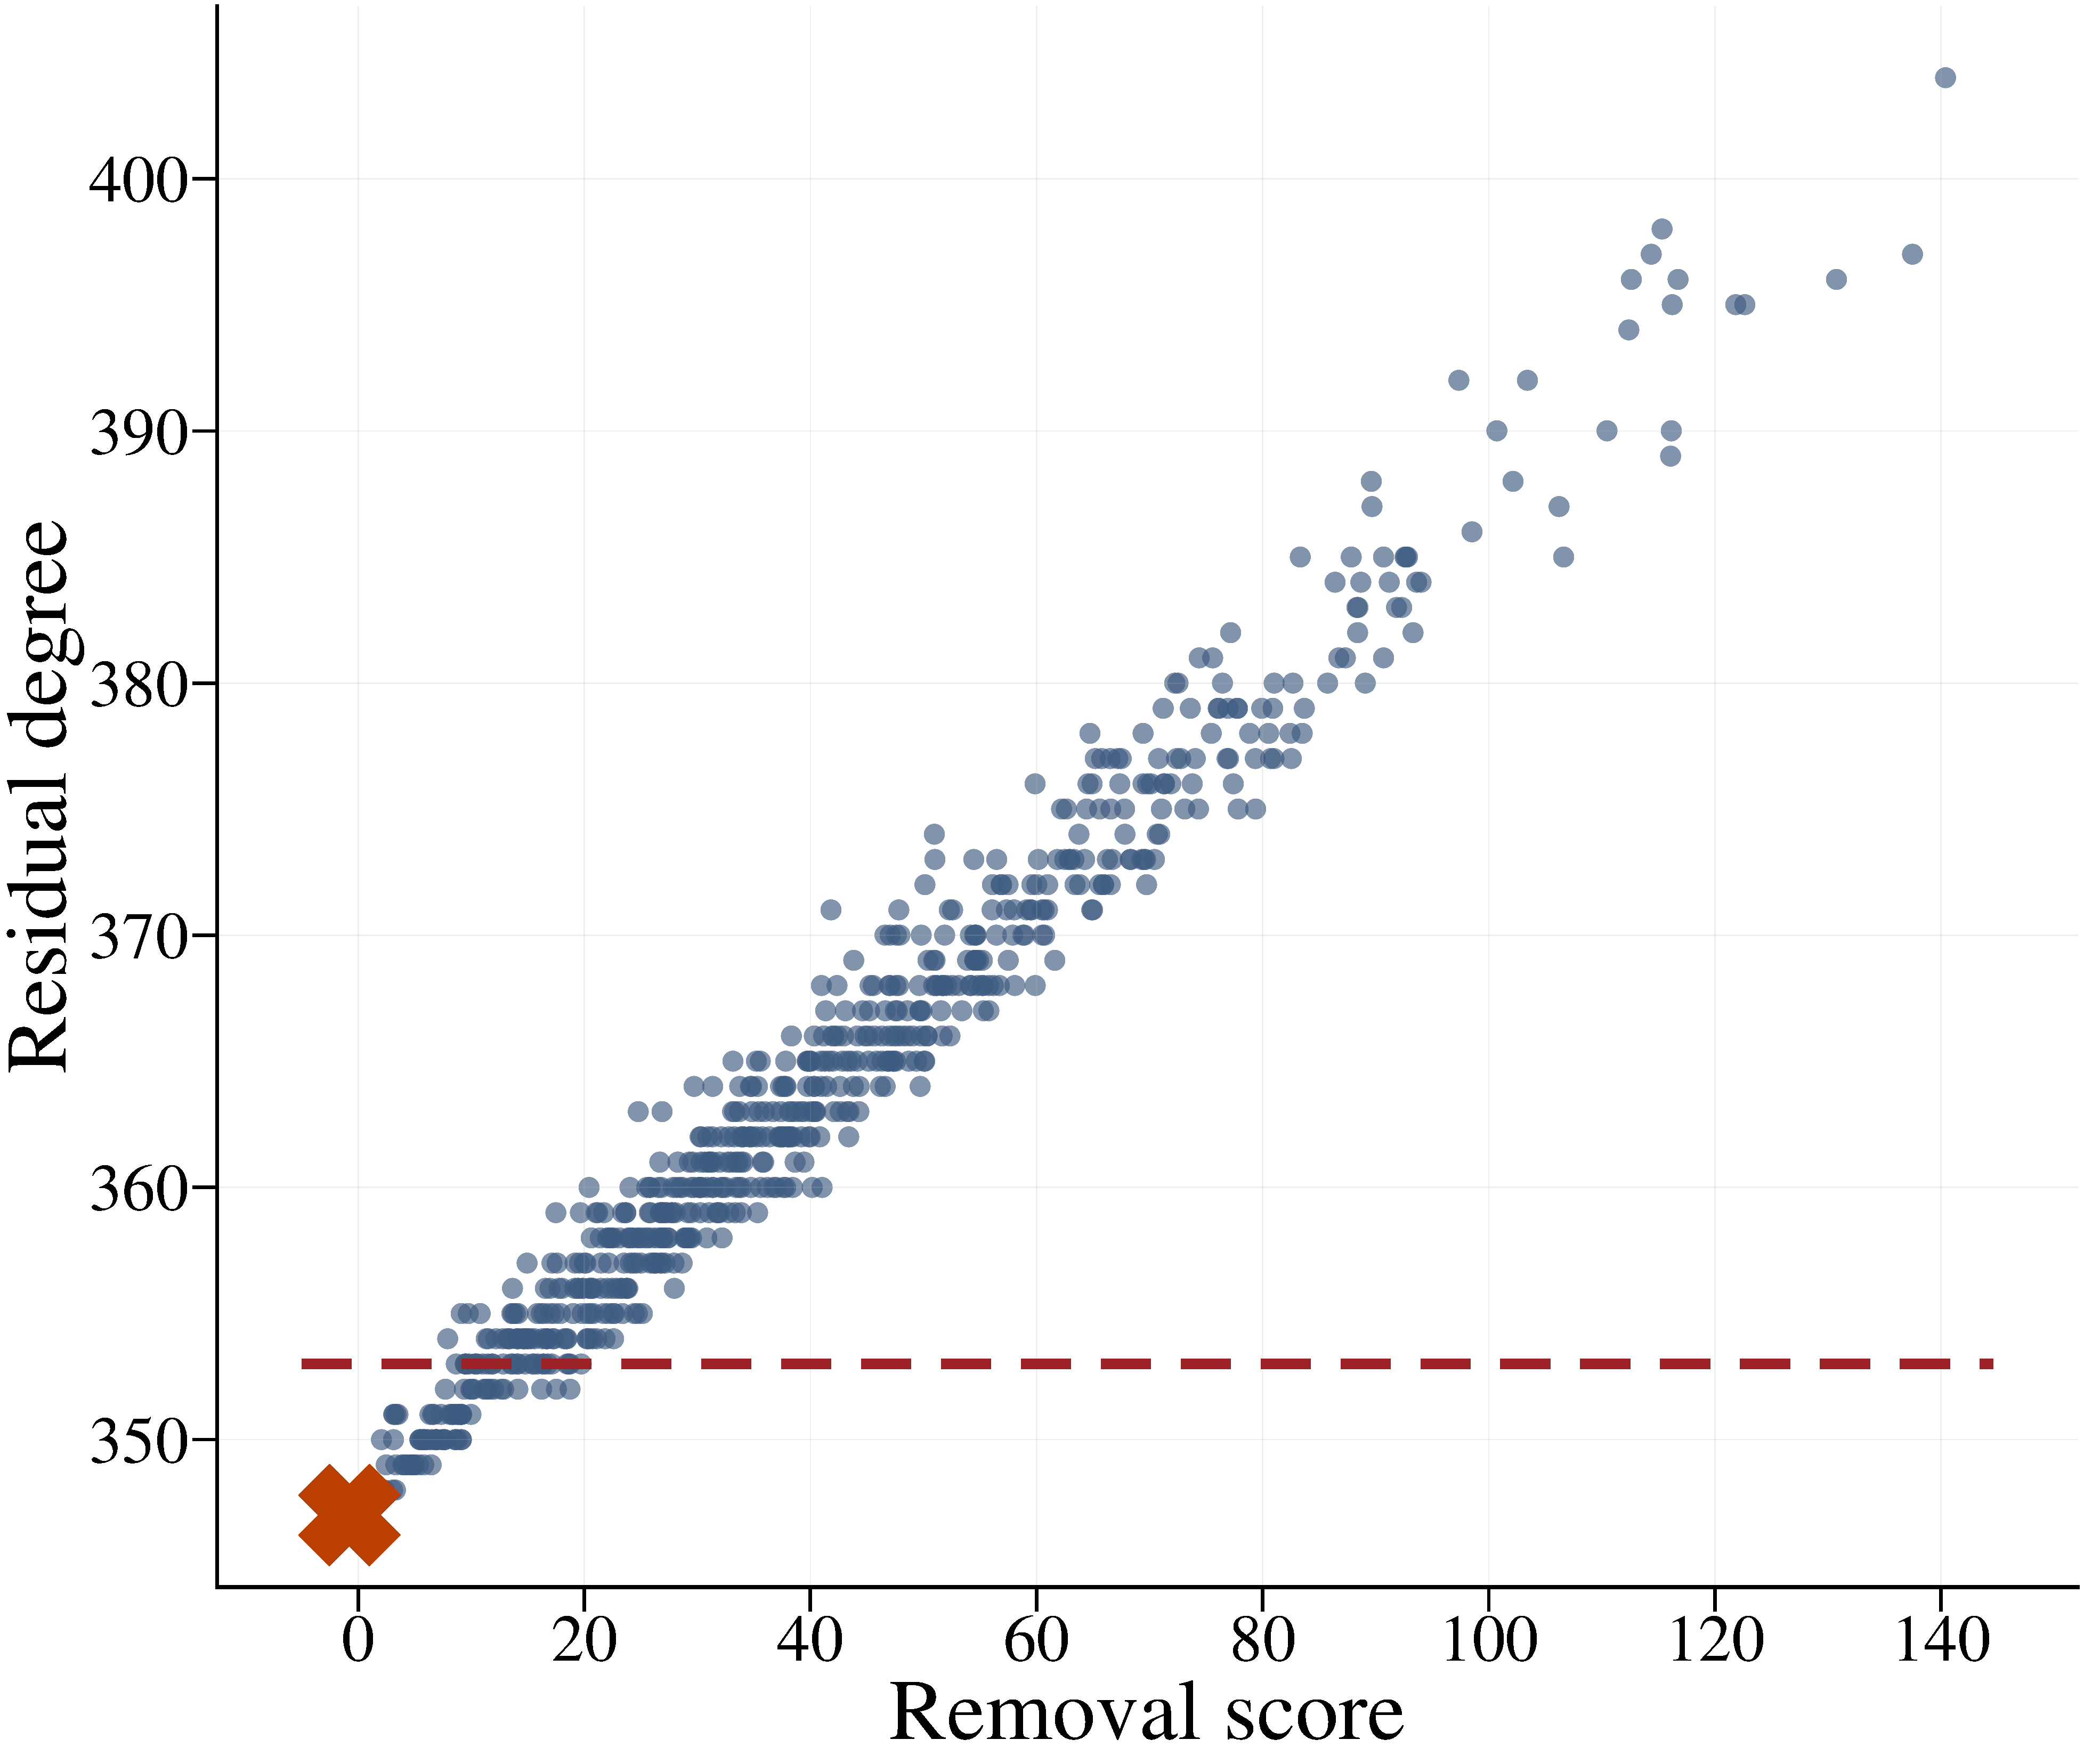
\includegraphics[width=0.38\textwidth]{SGNN_GU_self_predictor_lpr_train_medium_g0_upr_step300_score_vs_degree.pdf}}
    \end{tabular}
  \end{adjustbox}
  \caption{Score--degree pruning decisions during U-LPR. Rows correspond to
    pruning iterations $t=0,5,300$; columns correspond to \textsc{SGNN+U} and
    \textsc{SGNN+GU}. Each panel plots updater score (horizontal) vs.\ residual
    degree (vertical). $\times$ marks the vertex selected for removal; dashed line
    marks the 15th-percentile degree threshold. \textsc{SGNN+GU} keeps the selected deletion
    below this threshold throughout pruning, whereas \textsc{SGNN+U} continues to select
  high-degree vertices.}
  \label{fig:score_degree_pruning_grid}
\end{figure}

% ================================================================
\subsection{Real-World Experiments}
\label{sec:realworld}
% ================================================================

The real-world results test whether the cached gradient remains useful outside the
planted-clique distribution. Table~\ref{tab:realworld} reports zero-shot U-LPR
performance on the six real-world datasets from Section~\ref{sec:realworld_data}. The SGNN Rerun column is the
$O(n^3)$ reference from~\citet{ShohamHRV26}; the U-LPR columns are new.

\begin{table}[H]
  \caption{Real-world performance across six graph benchmarks (see
    Table~\ref{tab:datasets} for dataset statistics), reported as mean$\pm$std.
    SGNN Rerun results ($\dagger$) are from~\citet{ShohamHRV26}
    and serve as the $O(n^3)$ reference. Our contribution is the SGNN+U U-LPR and
    SGNN+GU U-LPR columns ($O(n^2)$). On structured datasets (IMDB Binary,
    com-youtube, com-orkut), \textsc{SGNN+GU} U-LPR approaches the rerun baseline;
    on heterogeneous graphs (Twitter, Facebook), a meaningful gap remains.
  $^\ddagger$Facebook results are indicative only ($n{=}10$ graphs).}
  \label{tab:realworld}
  \resizebox{\textwidth}{!}{%
    \begin{tabular}{lrrccccccccc}
      \toprule
      & & & \multicolumn{3}{c}{SGNN Rerun$^\dagger$ [$O(n^3)$]}
      & \multicolumn{3}{c}{\textsc{SGNN+U} U-LPR [$O(n^2)$]}
      & \multicolumn{3}{c}{\textsc{SGNN+GU} U-LPR [$O(n^2)$]} \\
      \cmidrule(lr){4-6}\cmidrule(lr){6-8}\cmidrule(lr){9-11}\cmidrule(lr){10-12}
      Dataset & Graphs & Avg.\,$n$ & Approx & Overlap & Exact
      & Approx & Overlap & Exact
      & Approx & Overlap & Exact \\
      \midrule
      Twitter       & 973   & $131{\pm}64$    & $0.977{\pm}0.051$ & $0.774{\pm}0.251$ & $0.228{\pm}0.420$
      & $0.214{\pm}0.160$ & $0.040{\pm}0.126$ & $0.009{\pm}0.096$
      & $0.830{\pm}0.233$ & $0.590{\pm}0.324$ & $0.088{\pm}0.284$ \\
      Collab        & 5000  & $74.5{\pm}62$   & $0.999{\pm}0.010$ & $0.969{\pm}0.142$ & $0.929{\pm}0.257$
      & $0.611{\pm}0.357$ & $0.434{\pm}0.433$ & $0.341{\pm}0.474$
      & $0.884{\pm}0.201$ & $0.803{\pm}0.295$ & $0.627{\pm}0.484$ \\
      IMDB Binary   & 1000  & $19.8{\pm}10$   & $1.000$            & $0.933{\pm}0.223$ & $0.914{\pm}0.281$
      & $0.980{\pm}0.077$ & $0.841{\pm}0.326$ & $0.802{\pm}0.399$
      & $0.997{\pm}0.038$ & $0.923{\pm}0.236$ & $0.901{\pm}0.299$ \\
      com-youtube   & 16386 & $7.8{\pm}42.2$  & $0.999{\pm}0.015$ & $0.924{\pm}0.208$ & $0.865{\pm}0.342$
      & $0.949{\pm}0.145$ & $0.834{\pm}0.322$ & $0.770{\pm}0.421$
      & $0.968{\pm}0.106$ & $0.857{\pm}0.289$ & $0.783{\pm}0.412$ \\
      com-orkut     & 5000  & $215{\pm}320$   & $0.969{\pm}0.057$ & $0.734{\pm}0.295$ & $0.183{\pm}0.387$
      & $0.902{\pm}0.217$ & $0.799{\pm}0.333$ & $0.687{\pm}0.464$
      & $0.937{\pm}0.187$ & $0.859{\pm}0.279$ & $0.747{\pm}0.435$ \\
      Facebook$^\ddagger$ & 10 & $416{\pm}329$ & $0.966{\pm}0.053$ & $0.688{\pm}0.342$ & $0.000$
      & $0.274{\pm}0.214$ & $0.091{\pm}0.104$ & $0.000$
      & $0.750{\pm}0.223$ & $0.311{\pm}0.325$ & $0.000$ \\
      \bottomrule
    \end{tabular}%
  }
  % \smallskip\par
  % \noindent\small $^\dagger$ Reproduced from~\citet{ShohamHRV26}.\quad
  % $^\ddagger$ Ten graphs only; interpret with caution.
\end{table}

\textsc{SGNN+GU} U-LPR substantially outperforms \textsc{SGNN+U} U-LPR.
On all six datasets, gradient injection brings a large improvement over the
score-only updater, confirming that the gradient channel is necessary for
incremental decoding even outside the planted-clique distribution.

A quality--efficiency gap remains on heterogeneous graphs.
On four of six datasets (IMDB Binary, com-youtube, com-orkut, and Collab),
\textsc{SGNN+GU} U-LPR approaches the rerun approximation ratio closely. On Twitter
and Facebook, however, a meaningful gap remains. Both datasets have pronounced hub
structure absent from planted-clique instances: Twitter's degree distribution is
power-law, and Facebook ego networks contain high-degree hubs by construction.
The gradient carries the correct residual signal, but $U_\theta$ struggles to learn
to exploit it precisely on these out-of-distribution structures. We discuss this
trade-off and a potential remedy in Section~\ref{sec:discussion}.

% ================================================================
\section{Discussion}
\label{sec:discussion}
% ================================================================

The central contribution of this paper is not the observation that gradients can be
useful to a neural decoder. Gradients are already used in many neural optimization
methods as search directions, training signals, or auxiliary features. Our use is
different. Here, the gradient is useful because it has a valid residual transition:
after deleting a vertex, its change can be written as an exact local correction. This
makes it a maintainable state variable for the residual graph.

This distinction is important because the failure mode is not poor initial scoring.
The backbone learns the expected degree-like ordering, and rerunning the GNN after
each deletion confirms that fresh neural scores can support strong pruning decisions.
The problem is that these scores are not themselves residual statistics. Once the
relevant information is represented through nonlinear activations such as $\tanh$ or
sigmoid, equal changes in the underlying graph need not correspond to equal changes
in the score. A score can therefore be accurate on the current graph while still
being unsuitable for local maintenance after the next deletion.

Gradient injection repairs this specific incompatibility. It does not make the GNN
more expressive, and it is not merely an extra feature appended to the updater. It
exposes a probability-space coordinate whose deletion dynamics remain local even
after the GNN score has passed through nonlinear layers. The learned updater can
then act on a live residual state instead of trying to reconstruct the missing
correction from stale post-activation scores. In this sense, the gradient channel is
a structural device: it restores the local update property that classical residual
heuristics have and nonlinear neural scores lack.

This also clarifies the role of SIT. The rerun teacher provides a target deletion
trajectory, but imitation alone does not make the trajectory maintainable. A
score-only updater can see the same teacher decisions and still fail, because its
state does not evolve consistently with the residual graph. With the cached
probability-space gradient, the student is given a coordinate system that can be
carried through the deletion process. SIT then teaches how to act on that coordinate;
it is not the source of update compatibility by itself.

The remaining gaps should be interpreted in the same terms. In the Hard regime,
rerunning the GNN can exploit signals that are useful on the current residual graph
but are not necessarily captured by the cached gradient used here. Thus update
compatibility is not the same as general residual intelligence: the gradient fixes a
specific nonlinearity-induced maintenance problem, but it does not guarantee that all
information available to a rerun decoder has been made incrementally accessible.
Similarly, on heterogeneous real-world graphs, the cached gradient remains useful
but does not fully close the gap to rerun decoding. This suggests that the next
question is not whether to ``use gradients'', but which residual coordinate has the
right local transition for the graph family and objective at hand.

More broadly, the design criterion suggested by these results is simple. A neural
residual decoder should expose not only a good score, but also a state variable whose
meaning survives the residual operation. For the clique objective, the
probability-space gradient satisfies this criterion because its deletion update is
local and exact. For other objectives, the same idea should be judged by the same
test: does the proposed signal have a valid local update rule, or is it only another
informative feature?

\subsection{Limitations and Future Work}

A first limitation is that the update-compatible coordinate is supplied manually. The
clique objective is known, so we can derive and maintain
$\nabla_p\mathcal{L}_{\mathrm{clique}}$ explicitly. This isolates the role of the
residual signal, but it is not yet a fully learned solution. A stronger approach
would learn locally maintainable coordinates directly, learn how to expose such
coordinates from the objective without hand-designing the cache, or use the gradient tracking capabilities of modern deep learning frameworks such as PyTorch or Tensorflow.

Second, exposing a valid residual coordinate does not guarantee that SGD will use it
correctly. SIT is needed because the architecture supplies a maintainable state, but
the updater must still learn which deletion decisions that state supports. Future
work should study objectives or architectures that make this behavior emerge without
requiring a rerun teacher.

Third, SIT has an offline distillation cost: the teacher reruns the GNN for $T=300$
deletion steps per instance, although inference after training is quadratic. It also
inherits the teacher's limitations. On instances where the rerun teacher is weak, the
student has limited targets to imitate. Shorter teacher horizons, sparse
distillation, or direct training from final clique quality are natural alternatives.

The Hard-regime gap remains an open question. On these instances,
\textsc{SGNN+U}+SIT with rerun decoding performs better than the maintainable
U-LPR variants, indicating that reruns may expose useful residual information not
captured by the current cached gradient. Future work should identify what this
information is and whether it can be represented by another locally maintainable
coordinate rather than by returning to cubic decoding.

A possible direction for the real-world gap on Twitter and Facebook is to test
alternative residual coordinates, including logit-space signals such as
$\nabla_z \mathcal{L}_{\mathrm{clique}} =
\nabla_p \mathcal{L}_{\mathrm{clique}} \odot p \odot (1-p)$. Such signals may behave
differently on graphs where score saturation differs from the planted-clique
distribution. Maintaining them incrementally would require a cache that also accounts
for the sigmoid derivative after each deletion.

Finally, the experiments focus on planted clique and on an objective whose gradient
has a simple cached form. Extending the approach to independent set,
constraint-satisfaction relaxations, or other locally decomposable objectives should
be possible when analogous local update rules exist. The more difficult question is
whether such coordinates can be found or learned for objectives whose residual
changes are less explicitly structured.

\section{Conclusions}
\label{sec:conclusions}

This paper identifies update compatibility as a separate requirement from score
quality in neural residual decoders. A GNN can learn an informative degree-like
ranking for \textsc{Max-Clique}, yet the resulting nonlinear score is not
automatically maintainable after vertex deletions. Injecting and incrementally
maintaining the probability-space objective gradient provides a residual coordinate
whose deletion update is local and exact. Empirically, this lets \textsc{SGNN+GU}
with Self-Imitation Training recover quadratic residual decoding while matching the
rerun baseline on Easy and Medium planted-clique instances and substantially
outperforming score-only incremental decoding on real-world graphs. The main design
lesson is that neural combinatorial solvers should expose quantities whose changes
remain locally maintainable, not only scores that are accurate before the residual
state changes.

% ================================================================
%  MDPI REQUIRED END-MATTER
% ================================================================

\authorcontributions{%
  Conceptualization, E.S.; methodology, E.S.; software, E.S.; validation, E.S.;
  formal analysis, E.S.; investigation, E.S.; writing---original draft preparation,
  E.S.; visualization, E.S.; writing---review and editing, E.S., H.R. and D.V.;
  supervision, H.R. and D.V.
  All authors have read and agreed to the published version of the manuscript.
}

\funding{This research received no external funding.}

\institutionalreview{Not applicable.}

\informedconsent{Not applicable.}

\dataavailability{%
  % Two categories of data are used. First, planted-clique instances are synthetically   generated from the distribution described in Section~\ref{sec:problem}; no   external source is required and results can be reproduced by regenerating instances according to the stated sampling protocol and difficulty ranges.  Second, the real-world graph benchmarks used in Section~\ref{sec:realworld} are  publicly available: Twitter, Collab, and IMDB Binary are available through the   TUDataset collection~\citep{Morris+2020}; com-youtube, com-orkut, and Facebook are available through the Stanford SNAP repository~\citep{datasets}. The code for instance generation, training, evaluation, and figure production will be   deposited in a public repository upon acceptance.
  The original data presented in this study are openly available. The synthetic planted-clique datasets and source code used for instance generation, training, evaluation, and figure production are available in the public repository \citep{n_squared_clique_repo}, \url{https://github.com/Laboratory-of-Computational-Insight/n_sqaured_clique}. The real-world graph benchmarks analyzed in this study are publicly available through the TUDataset repository \citep{Morris+2020}, \url{https://chrsmrrs.github.io/datasets/}, and the Stanford SNAP repository \citep{datasets}, \url{https://snap.stanford.edu/data/}.
}

\acknowledgments{%
  During the preparation of this manuscript, the authors used OpenAI ChatGPT
  (GPT-5.5 Thinking, accessed May 2026) for grammar, spelling, and language
  editing. The first schematic figure was edited with AI assistance. The authors
  reviewed and edited the output and take full responsibility for the content of
  this publication.
}

\conflictsofinterest{The authors declare no conflicts of interest.}

% ================================================================
%  ABBREVIATIONS
% ================================================================
\abbreviations{Abbreviations}{%
  The following abbreviations are used in this manuscript:\\
  \noindent
  \begin{tabular}{@{}ll}
    GNN     & Graph Neural Network \\
    MPNN    & Message-Passing Neural Network \\
    MLP     & Multi-Layer Perceptron \\
    LDR   & Least Degree Removal \\
    LPR   & Least Probable Removal \\
    U-LPR   & Updatable Least Probable Removal \\
    SIT     & Self-Imitation Training \\
    OBJ     & Objective (training regime) \\
    \textsc{SGNN}    & Standard GNN (backbone only) \\
    \textsc{SGNN+U}  & \textsc{SGNN} with score updater, no gradient channel \\
    \textsc{SGNN+GU} & \textsc{SGNN} with score updater and gradient channel \\
    WL      & Weisfeiler--Leman (graph isomorphism test) \\
    SDP     & Semidefinite Program \\
    UGC     & Unique Games Conjecture \\
    PC1/PC2 & First/Second Principal Component \\
  \end{tabular}
}

% ================================================================
\bibliography{bib}

% ================================================================
\clearpage
\appendixtitles{yes}
\appendix

% ================================================================
\section{Algorithms}
\label{app:algorithms}
% ================================================================

\begin{algorithm}[H]
  \caption{U-LPR: Cached-Deletion Decoder}
  \label{alg:gub}
  \begin{algorithmic}[1]
    \State Run GNN once to obtain scores $s_i$ and probabilities $p_i$ for all $i$.
    \State Initialize gradient/cache from $p$. \hfill\Comment{$O(n^2)$}
    \State $C \leftarrow V(G)$.
    \While{$C$ does not form a clique}
    \State $v^* \leftarrow \arg\min_{i \in C} s_i$;\;
    $C \leftarrow C \setminus \{v^*\}$.
    \State Remove $v^*$'s contribution from gradient cache. \hfill\Comment{$O(n)$}
    \State $g_i \leftarrow$ gradient from updated cache for all $i \in C$.
    \hfill\Comment{$O(n)$}
    \State $s_i \mathrel{+}= U_\theta(s_i,\, s_{v^*},\, A_{iv^*},\, g_i,\,
    g_{v^*})$ for all $i \in C$. \hfill\Comment{$O(n)$}
    \EndWhile
    \State \Return $C$.
  \end{algorithmic}
\end{algorithm}

\begin{algorithm}[H]
  \caption{SIT Training Step}
  \label{alg:sit_training}
  \begin{algorithmic}[1]
    \State Sample instance $(G, k)$; run GNN once to obtain $\tilde{s}$, $p$.
    \State Initialize gradient/cache from $p$.
    \hfill\Comment{$O(n^2)$; \textsc{SGNN+GU} only}
    \For{$t = 0, \ldots, T-1$}
    \State $v^t_{\mathrm{teach}} \leftarrow \arg\min_{i \in V(G_t)}
    \mathrm{GNN}(G_t)_i$. \hfill\Comment{Teacher reruns GNN, $O(n^2)$}
    \State $\mathcal{L}_{\mathrm{SIT}} \mathrel{+}=
    \mathrm{CE}_{\mathrm{softmax}}(-\tilde{s}_{V(G_t)},\,
    v^t_{\mathrm{teach}})$.
    \hfill\Comment{Student predicts same removal}
    \State $G_t \leftarrow G_t \setminus \{v^t_{\mathrm{teach}}\}$.
    \State Update gradient cache by removing $v^t_{\mathrm{teach}}$.
    \hfill\Comment{$O(n)$; \textsc{SGNN+GU} only}
    \State $\tilde{s}_i \mathrel{+}= U_\theta(\tilde{s}_i,\,
    \tilde{s}_{v^t},\, A_{iv^t},\, \gamma_i,\, \gamma_{v^t})$
    for all $i \in V(G_t)$.
    \EndFor
    \State Optimise $\mathcal{L}_{\mathrm{clique}} +
    \mathcal{L}_{\mathrm{SIT}} / T$.
  \end{algorithmic}
\end{algorithm}

% ================================================================
\section{Formal Claims and Proofs}
\label{app:proofs}
% ================================================================

This appendix contains the formal statements and proofs of the observations
summarised in Section~\ref{sec:theory}.

\begin{claim}[Affine requirement for additive updates]
  \label{claim:affine_needed}
  Let $d$ be a scalar maintained statistic, and suppose deleting a neighboring vertex
  changes $d$ to $d-1$. If a score $r(d)$ admits an exact deletion update of the form
  \[
    r(d-1)=r(d)-c
  \]
  with the same constant $c$ for all values of $d$, then $r$ is affine on the
  reachable values of $d$. In particular, a nonlinear activation such as $\tanh$ or
  sigmoid cannot support a fixed additive correction on any interval where its
  discrete differences are not constant.
\end{claim}

\begin{proof}
  For every reachable integer $d$, the assumed update rule gives
  \[
    r(d)-r(d-1)=c .
  \]
  Thus all first discrete differences of $r$ are equal. By summing these differences,
  for any $d>d_0$ we obtain
  \[
    r(d)=r(d_0)+c(d-d_0),
  \]
  so $r$ is affine on the reachable domain. Nonlinear activations violate this
  condition. For example,
  \[
    \tanh(6)-\tanh(5) \neq \tanh(2)-\tanh(1),
  \]
  so a post-activation score cannot be updated exactly by subtracting a single fixed
  constant after each unit change in the underlying statistic.
\end{proof}

\begin{claim}[Ordering instability under approximate scores]
  \label{claim:ordering_instability}
  Let an exact residual decoder remove vertices in order of increasing score
  $r_t(i)$, and let an approximate decoder use scores
  $\tilde r_t(i)=r_t(i)+e_t(i)$ where $|e_t(i)|\le\varepsilon$ for all $i$. If
  at some step $t$ there exist alive vertices $i,j$ with score gap
  \[
    0 < r_t(i)-r_t(j) < 2\varepsilon,
  \]
  then the errors $e_t(i)=-\varepsilon$, $e_t(j)=+\varepsilon$ reverse their
  order under the approximate decoder. After such a reversal, the two decoders
  continue on different residual graphs, so later scores are no longer
  perturbations of the same state.
\end{claim}

\begin{proof}
  Choose errors $e_t(i)=-\varepsilon$ and $e_t(j)=+\varepsilon$. Then
  \[
    \tilde r_t(i)-\tilde r_t(j)
    =
    r_t(i)-r_t(j)-2\varepsilon
    <0,
  \]
  so the approximate decoder ranks $i$ below $j$ although the exact decoder ranks
  $j$ below $i$. If one decoder deletes $i$ and the other deletes $j$, the alive sets
  become different. Since all later residual scores are functions of the alive set,
  subsequent discrepancies are structural rather than merely numerical. Thus local
  score-update error can change the deletion trajectory, and a decoder that lacks an
  exact maintainable state has no general guarantee of staying aligned with the
  rerun decoder.
\end{proof}

\begin{claim}[Local gradient update]
  \label{claim:local_gradient}
  For the clique objective~\eqref{eq:clique_loss}, deleting a vertex $v$ changes each
  surviving gradient coordinate by a local correction depending only on $A_{iv}$,
  $B_{iv}$, and $p_v$. Specifically, if
  \[
    g_i=-2(Ap)_i+2(Bp)_i,
  \]
  then after deleting $v$,
  \[
    g_i' = g_i + 2A_{iv}p_v - 2B_{iv}p_v,
    \qquad i\neq v.
  \]
\end{claim}

\begin{proof}
  Before deletion,
  \[
    g_i=-2\sum_{j\in S} A_{ij}p_j
    +2\sum_{j\in S} B_{ij}p_j .
  \]
  After deleting $v$, the alive set becomes $S'=S\setminus\{v\}$ and $p_v$ is set to
  zero. Hence
  \[
    g_i'
    =
    -2\sum_{j\in S'} A_{ij}p_j
    +2\sum_{j\in S'} B_{ij}p_j .
  \]
  Subtracting the two expressions removes exactly the terms involving $v$:
  \[
    g_i'-g_i
    =
    2A_{iv}p_v - 2B_{iv}p_v .
  \]
  This correction is local: it depends only on whether $i$ is adjacent to the deleted
  vertex, whether it is a non-neighbor, and the deleted vertex probability.
\end{proof}

\begin{claim}[Cached maintenance complexity]
  \label{claim:cache_complexity}
  The gradient cache for~\eqref{eq:clique_gradient} can be initialized in $O(n^2)$
  time and updated in $O(n)$ time per deletion. Therefore U-LPR with cached gradients
  has $O(n^2)$ total cache-maintenance cost after the initial GNN pass.
\end{claim}

\begin{proof}
  Initialize
  \[
    a=Ap,\qquad b=Bp,
  \]
  by two matrix-vector products, which cost $O(n^2)$ on dense graphs. When vertex
  $v$ is deleted, update each surviving coordinate by
  \[
    a_i \leftarrow a_i-A_{iv}p_v,
    \qquad
    b_i \leftarrow b_i-B_{iv}p_v .
  \]
  This is one column subtraction for $A$ and one for $B$, hence $O(n)$ time. Since at
  most $n$ vertices are deleted, all updates together cost $O(n^2)$. The gradient
  itself is then recovered as $g=-2a+2b$ on the alive coordinates, also in $O(n)$ per
  step.
\end{proof}

% ================================================================
\section{Scaling Experiments}
\label{app:scaling}
% ================================================================

Table~\ref{tab:scaling} reports wall-clock decoding time across
$n\in\{500,1000,1500,2000,5000\}$ for all three models and decoders. The speedup
of \textsc{SGNN+GU} U-LPR over Rerun is about $1.5\times$ at $n=1000$ and
$1.7\times$ at $n=5000$. At $n=2000$, \textsc{SGNN+GU} U-LPR ($5.873\pm1.182$\,s)
and Rerun ($5.912\pm0.909$\,s) differ by under $0.04$\,s, well within one standard
deviation of either measurement; this reflects timing noise rather than a reversal
of the trend. The current architecture uses a lightweight backbone ($L=4$, hidden
dimension 64) and a fixed-width updater, so constant factors from dense matrix
operations dominate at these graph sizes. The asymptotic advantage of $O(n^2)$ over
$O(n^3)$ is expected to become more pronounced at larger $n$ and with deeper
backbones, as rerun cost grows cubically while updater cost grows quadratically.
Note also that \textsc{SGNN+U} U-LPR is faster than \textsc{SGNN+GU} U-LPR at
all sizes (e.g., $8.2$\,s vs $11.4$\,s at $n=5000$) because it omits the gradient
cache; however, \textsc{SGNN+U} U-LPR fails on Medium instances (Table~1), so this
speed advantage comes at a significant quality cost.

\begin{table}[H]
  \caption{Wall-clock time (seconds per instance) across graph sizes
    $n\in\{500,1000,1500,2000,5000\}$, mean$\pm$std over held-out instances.
  The $n=1000$ row corresponds to Table~\ref{tab:timing} in the main text.}
  \label{tab:scaling}
  \centering
  \resizebox{\textwidth}{!}{%
    \begin{tabular}{lrrrr}
      \toprule
      Model & $n$ & Top-$k$ (s) & Rerun (s) & U-LPR (s) \\
      \midrule
      \multirow{4}{*}{\textsc{SGNN} + OBJ}
      & 500  & $0.183\pm0.123$ & $1.381\pm0.170$ & --- \\
      & 1000 & $0.093\pm0.037$ & $1.027\pm0.018$ & --- \\
      & 1500 & $0.510\pm0.120$ & $4.304\pm0.428$ & --- \\
      & 2000 & $0.780\pm0.121$ & $6.302\pm0.793$ & --- \\
      & 5000 & $1.248\pm0.418$ & $19.261\pm0.375$ & --- \\
      \midrule
      \multirow{5}{*}{\textsc{SGNN+U} + SIT}
      & 500  & $0.157\pm0.053$ & $1.393\pm0.170$ & $0.978\pm0.195$ \\
      & 1000 & $0.078\pm0.003$ & $1.044\pm0.084$ & $0.492\pm0.026$ \\
      & 1500 & $0.512\pm0.161$ & $4.215\pm0.450$ & $2.556\pm0.358$ \\
      & 2000 & $0.731\pm0.132$ & $5.951\pm0.706$ & $3.931\pm0.617$ \\
      & 5000 & $1.657\pm0.161$ & $19.327\pm0.706$ & $8.187\pm0.703$ \\
      \midrule
      \multirow{5}{*}{\textsc{SGNN+GU} + SIT}
      & 500  & $0.190\pm0.036$ & $1.328\pm0.168$ & $1.146\pm0.218$ \\
      & 1000 & $0.079\pm0.003$ & $1.031\pm0.046$ & $0.675\pm0.012$ \\
      & 1500 & $0.469\pm0.119$ & $4.288\pm0.418$ & $3.937\pm0.667$ \\
      & 2000 & $0.732\pm0.195$ & $5.912\pm0.909$ & $5.873\pm1.182$ \\
      & 5000 & $1.431\pm0.253$ & $19.269\pm0.326$ & $11.401\pm1.952$ \\
      \bottomrule
    \end{tabular}%
  }
\end{table}

\end{document}
